\chapter{Power/EM I} \label{c4_forthchapter:cha}

In this chapter, we're going to learn about:
\begin{itemize}
    \item Electric Engineering basics
    \item When \& Where in an electronic circuit is power consumed
    \item How can we measure power \& EM consumption?
\end{itemize}

\section{Electronic Circuits 101}

\subsection{A basic electronic circuit}

The most basic electronic circuit (Figure \ref{fig:basic_electronic_circuitn}) consists of a power supply (Vdd)
and some sort of electrical load (a component consuming electric power)
connected to the power supply on the one hand and to the ``ground" (the reference point from which electric potential or voltage is measured) on the other hand. As the electric current - a targeted flow of free electrons -
flows through the load, the load does some kind of a ``work''. We can think of electric
current as behaving like water - going from the hill (Vdd) to the valey (Ground) with rivers and obstacles (Loads/Resistors) trying to prevent it from flowing. The higher the resistance of the load, the less current will be able to flow through it.

\begin{figure}[!ht]
	\centering
	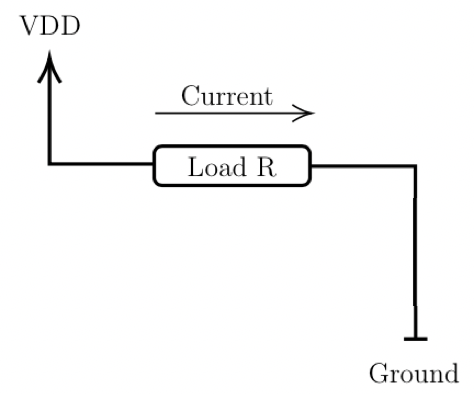
\includegraphics{images/basic_electronic_circuit.png}
	\caption{Basic electronic circuit.} \label{fig:basic_electronic_circuitn}
\end{figure}


There are two different ways to wire different loads on an electric circuit - "in series" and "in parallel":
\begin{itemize}
    \item \textbf{In series} - electricity has to pass through one load to reach the other.
    \item \textbf{In parallel} - the loads are conected side by side and the electric current passes through them in parallel.
\end{itemize}

The electric potential difference between the power supply and the ground creates an
electric current which flows through the load toward the ground. The difference
in electric potential between two points is measured in Volts (usually denoted
by \textbf{\textit{V}}). The magnitude of the current flowing through the circuit at a
given time is measured in Amperes (denoted by \textbf{\textit{A}}). The
electrical resistance of the load is a measure of its opposition to the flow of
electric current through it. It is measured in Ohms (and denoted by
\textbf{\textit{R}}).

\subsection{Resistors}

As the name implies, a resistor resists the flow of electrical current. The
amount of resistance is measured in Ohms. A resistor is considered a passive
component that consumes power that is dissipated as heat. The power rating of a
resistor determines how much power it can consume without overheating.

\begin{figure}[!ht]
    \centering
    \tikzset{every picture/.style={line width=0.75pt}} %set default line width to 0.75pt        

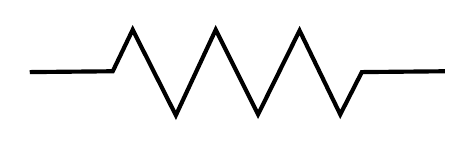
\begin{tikzpicture}[x=0.75pt,y=0.75pt,yscale=-1,xscale=1]
%uncomment if require: \path (0,82); %set diagram left start at 0, and has height of 82

%Straight Lines [id:da11666992549989796] 
\draw [line width=1.5]    (11.4,40.02) -- (51.4,39.62) -- (61,19.62) -- (81.8,60.82) -- (101,19.62) -- (121.4,60.42) -- (141.4,20.02) -- (161,60.42) -- (171.4,40.02) -- (211.4,39.62) ;






\end{tikzpicture}
    \caption{Resistor Symbol in Circuit Diagrams.} \label{fig:resistor}
\end{figure}

\subsection{Ohm's law}

\begin{figure}[!ht]
	\centering
	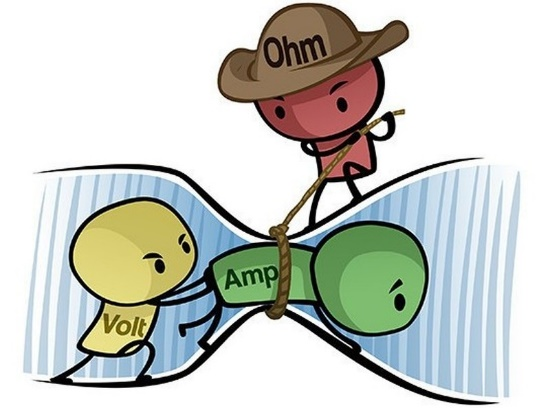
\includegraphics{images/ohms_law_cartoon.png}
	\caption{Ohm's Law.} \label{fig:ohms_law_cartoon}
\end{figure}

Ohm's law defines the relationship between the Voltage, Current and Resistance
in a circuit: The voltage is equal to the current multiplied by the resistance
of the load. 

\begin{displaymath}\label{eq:ohm}
    V=I \cdot R
\end{displaymath}

Since in most of the circuits we are using, the voltage is fixed (defined by the
characteristics of the power supply), a change in the resistance of the circuit
will cause an inverse change in the current. A useful
analogy for the relations between V, I and R is to imagine a fountain springing from a high
mountain with water flowing down through a river to the sea. The difference
in height between the fountain and the sea is the Voltage, the width of the
river can be thought of as the resistance, and the flow of the water is the
current.

\subsection{Power}

Power is the rate at which work is done by the circuit and is measured in Watts.
Electricity bills are measured in units of Kilo-Watt x hour, i.e. 1 KWH is 1,000 watts used
for an hour, and this is the energy that we used and we need to pay for. 

\begin{displaymath}\label{eq:power_consumption}
    Power = \frac{Work}{Time}
\end{displaymath}

As an example we can consider a smartphone: the battery's capacity is measured in milli-Ampere hour (mAh).
So, if a battery has 3000 mAh of capacity, and the phone's basline power consumption is 1A  then we can use it
for 3 hours without recharging. Of course, if we overload the phone by watching videos on youtube (requires cpu/gpu for decoding, wifi/mobile for downloading content, etc.)
turning the flashlight on and so forth - then the power consumption would be higher and the battery will run out quicker. 

Different types of work can be done using electricity
\begin{itemize}
    \item Electromagnetic work (light a bulb, transmit a Wi-Fi signal)
    \item Thermal work (heating)
    \item Mechanical work (spin a motor, vibrate a speaker's diaphragm to play sounds)
    \item Chemical work (charging a battery)
    \item Computational work (store or load from memory, compute a value)
\end{itemize}

\subsection{Power Consumption}

When the current leaves the circuit to the ground then we consume it as power,
but sometimes we need to be careful as there are cases where the current is not really
leaving the circuit, like battery charging. In order to measure the power consumption we
will connect our measurement device between the load and the ground. The power
consumption of a device is the work it does divided by time. It is measured in
Watts (\textbf{\textit{W}}). The power consumption can also be calculated as current
(\textbf{\textit{I}}) multiplied by Voltage (\textbf{\textit{V}}): $P = I \cdot V$

\subsection{Current and Voltage dividers}
Before we take a look at two simple electronic circuits, we need to introduce
two additional terms: A \textbf{short (closed) circuit} is a piece of wire with
(almost) zero resistance. The circuit is in a closed state and there is
electric current flowing through the circuit, simply stated - it "works" as normal. An \textbf{open
circuit} is a circuit which doesn't allow any current to pass through it. The
circuit is in an open state and there is no current in the circuit. That's to
say - it doesn't ``work''.

\begin{figure}[!ht]
    \centering
    

\tikzset{every picture/.style={line width=0.75pt}} %set default line width to 0.75pt        

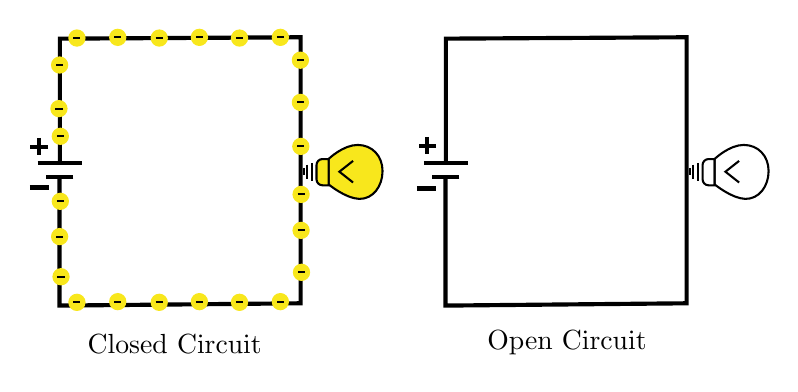
\begin{tikzpicture}[x=0.75pt,y=0.75pt,yscale=-1,xscale=1]
%uncomment if require: \path (0,199.3333282470703); %set diagram left start at 0, and has height of 199.3333282470703

%Straight Lines [id:da2325261898014528] 
\draw [color={rgb, 255:red, 0; green, 0; blue, 0 }  ,draw opacity=1 ][line width=1.5]    (35.5,90.67) -- (35.5,152.67) -- (151.67,151.56) -- (151.67,23.39) -- (35.67,24.06) -- (35.67,84.06) ;

\draw [shift={(35.5,90.67)}, rotate = 270] [color={rgb, 255:red, 0; green, 0; blue, 0 }  ,draw opacity=1 ][line width=1.5]    (0,6.71) -- (0,-6.71)   ;
%Straight Lines [id:da28409341931115617] 
\draw [color={rgb, 255:red, 0; green, 0; blue, 0 }  ,draw opacity=1 ][line width=1.5]    (25,84.06) -- (46.33,84.06) ;


%Shape: Polygon Curved [id:ds5857087256403513] 
\draw  [fill={rgb, 255:red, 248; green, 231; blue, 28 }  ,fill opacity=1 ] (165.14,94.26) .. controls (165.14,94.26) and (173.39,101.09) .. (179.94,101.26) .. controls (186.5,101.42) and (191.14,95.16) .. (191.14,87.86) .. controls (191.15,80.56) and (186.14,75.26) .. (179.14,75.26) .. controls (172.14,75.26) and (165.12,82.03) .. (165.14,82.06) .. controls (165.17,82.08) and (165.14,94.26) .. (165.14,94.26) -- cycle ;
%Rounded Same Side Corner Rect [id:dp42554815939285007] 
\draw  [fill={rgb, 255:red, 248; green, 231; blue, 28 }  ,fill opacity=1 ] (162.24,94.72) .. controls (160.63,94.72) and (159.33,93.42) .. (159.33,91.82) -- (159.33,84.96) .. controls (159.33,83.36) and (160.63,82.06) .. (162.24,82.06) -- (165.14,82.06) .. controls (165.14,82.06) and (165.14,82.06) .. (165.14,82.06) -- (165.14,94.72) .. controls (165.14,94.72) and (165.14,94.72) .. (165.14,94.72) -- cycle ;
%Straight Lines [id:da9150604099279609] 
\draw [line width=0.75]    (156.94,83.96) -- (156.94,92.56) ;


%Straight Lines [id:da28384528220983696] 
\draw [line width=0.75]    (154.94,84.76) -- (154.94,91.56) ;


%Straight Lines [id:da8752324892632142] 
\draw [line width=0.75]    (153.34,86.36) -- (153.34,89.56) ;


%Straight Lines [id:da25290786107493535] 
\draw [line width=0.75]    (176.94,82.96) -- (170.34,88.16) -- (176.94,93.36) ;


%Straight Lines [id:da9185196513242853] 
\draw [line width=1.5]    (21.17,95.78) -- (30.5,95.78) ;


%Shape: Circle [id:dp23397738064818174] 
\draw  [draw opacity=0][fill={rgb, 255:red, 248; green, 231; blue, 28 }  ,fill opacity=1 ] (147.6,75.97) .. controls (147.6,73.67) and (149.47,71.8) .. (151.77,71.8) .. controls (154.07,71.8) and (155.93,73.67) .. (155.93,75.97) .. controls (155.93,78.27) and (154.07,80.13) .. (151.77,80.13) .. controls (149.47,80.13) and (147.6,78.27) .. (147.6,75.97) -- cycle ;
%Straight Lines [id:da482836286674198] 
\draw    (150.05,75.97) -- (153.48,75.97) ;



%Shape: Circle [id:dp7549375095754003] 
\draw  [draw opacity=0][fill={rgb, 255:red, 248; green, 231; blue, 28 }  ,fill opacity=1 ] (147.4,54.77) .. controls (147.4,52.47) and (149.27,50.6) .. (151.57,50.6) .. controls (153.87,50.6) and (155.73,52.47) .. (155.73,54.77) .. controls (155.73,57.07) and (153.87,58.93) .. (151.57,58.93) .. controls (149.27,58.93) and (147.4,57.07) .. (147.4,54.77) -- cycle ;
%Straight Lines [id:da4285424058101477] 
\draw    (149.85,54.77) -- (153.28,54.77) ;



%Shape: Circle [id:dp5457818708688953] 
\draw  [draw opacity=0][fill={rgb, 255:red, 248; green, 231; blue, 28 }  ,fill opacity=1 ] (147.4,34.43) .. controls (147.4,32.13) and (149.27,30.27) .. (151.57,30.27) .. controls (153.87,30.27) and (155.73,32.13) .. (155.73,34.43) .. controls (155.73,36.73) and (153.87,38.6) .. (151.57,38.6) .. controls (149.27,38.6) and (147.4,36.73) .. (147.4,34.43) -- cycle ;
%Straight Lines [id:da8515924061724973] 
\draw    (149.85,34.43) -- (153.28,34.43) ;



%Shape: Circle [id:dp4359422667224846] 
\draw  [draw opacity=0][fill={rgb, 255:red, 248; green, 231; blue, 28 }  ,fill opacity=1 ] (137.73,23.43) .. controls (137.73,21.13) and (139.6,19.27) .. (141.9,19.27) .. controls (144.2,19.27) and (146.07,21.13) .. (146.07,23.43) .. controls (146.07,25.73) and (144.2,27.6) .. (141.9,27.6) .. controls (139.6,27.6) and (137.73,25.73) .. (137.73,23.43) -- cycle ;
%Straight Lines [id:da45892746068057066] 
\draw    (140.19,23.43) -- (143.61,23.43) ;



%Shape: Circle [id:dp10968014625901534] 
\draw  [draw opacity=0][fill={rgb, 255:red, 248; green, 231; blue, 28 }  ,fill opacity=1 ] (118.07,23.77) .. controls (118.07,21.47) and (119.93,19.6) .. (122.23,19.6) .. controls (124.53,19.6) and (126.4,21.47) .. (126.4,23.77) .. controls (126.4,26.07) and (124.53,27.93) .. (122.23,27.93) .. controls (119.93,27.93) and (118.07,26.07) .. (118.07,23.77) -- cycle ;
%Straight Lines [id:da5692830288753206] 
\draw    (120.52,23.77) -- (123.95,23.77) ;



%Shape: Circle [id:dp43116716627713836] 
\draw  [draw opacity=0][fill={rgb, 255:red, 248; green, 231; blue, 28 }  ,fill opacity=1 ] (98.73,23.43) .. controls (98.73,21.13) and (100.6,19.27) .. (102.9,19.27) .. controls (105.2,19.27) and (107.07,21.13) .. (107.07,23.43) .. controls (107.07,25.73) and (105.2,27.6) .. (102.9,27.6) .. controls (100.6,27.6) and (98.73,25.73) .. (98.73,23.43) -- cycle ;
%Straight Lines [id:da7403562369362462] 
\draw    (101.19,23.43) -- (104.61,23.43) ;



%Shape: Circle [id:dp03302036024104882] 
\draw  [draw opacity=0][fill={rgb, 255:red, 248; green, 231; blue, 28 }  ,fill opacity=1 ] (79.4,23.77) .. controls (79.4,21.47) and (81.27,19.6) .. (83.57,19.6) .. controls (85.87,19.6) and (87.73,21.47) .. (87.73,23.77) .. controls (87.73,26.07) and (85.87,27.93) .. (83.57,27.93) .. controls (81.27,27.93) and (79.4,26.07) .. (79.4,23.77) -- cycle ;
%Straight Lines [id:da40757318650872465] 
\draw    (81.85,23.77) -- (85.28,23.77) ;



%Shape: Circle [id:dp8000122366529838] 
\draw  [draw opacity=0][fill={rgb, 255:red, 248; green, 231; blue, 28 }  ,fill opacity=1 ] (59.4,23.43) .. controls (59.4,21.13) and (61.27,19.27) .. (63.57,19.27) .. controls (65.87,19.27) and (67.73,21.13) .. (67.73,23.43) .. controls (67.73,25.73) and (65.87,27.6) .. (63.57,27.6) .. controls (61.27,27.6) and (59.4,25.73) .. (59.4,23.43) -- cycle ;
%Straight Lines [id:da0875021467717878] 
\draw    (61.85,23.43) -- (65.28,23.43) ;



%Shape: Circle [id:dp05690070919084467] 
\draw  [draw opacity=0][fill={rgb, 255:red, 248; green, 231; blue, 28 }  ,fill opacity=1 ] (39.73,23.77) .. controls (39.73,21.47) and (41.6,19.6) .. (43.9,19.6) .. controls (46.2,19.6) and (48.07,21.47) .. (48.07,23.77) .. controls (48.07,26.07) and (46.2,27.93) .. (43.9,27.93) .. controls (41.6,27.93) and (39.73,26.07) .. (39.73,23.77) -- cycle ;
%Straight Lines [id:da5744558280008554] 
\draw    (42.19,23.77) -- (45.61,23.77) ;



%Shape: Circle [id:dp09815936705452866] 
\draw  [draw opacity=0][fill={rgb, 255:red, 248; green, 231; blue, 28 }  ,fill opacity=1 ] (31.4,36.77) .. controls (31.4,34.47) and (33.27,32.6) .. (35.57,32.6) .. controls (37.87,32.6) and (39.73,34.47) .. (39.73,36.77) .. controls (39.73,39.07) and (37.87,40.93) .. (35.57,40.93) .. controls (33.27,40.93) and (31.4,39.07) .. (31.4,36.77) -- cycle ;
%Straight Lines [id:da1455188221370589] 
\draw    (33.85,36.77) -- (37.28,36.77) ;



%Shape: Circle [id:dp898572524230915] 
\draw  [draw opacity=0][fill={rgb, 255:red, 248; green, 231; blue, 28 }  ,fill opacity=1 ] (31.07,57.77) .. controls (31.07,55.47) and (32.93,53.6) .. (35.23,53.6) .. controls (37.53,53.6) and (39.4,55.47) .. (39.4,57.77) .. controls (39.4,60.07) and (37.53,61.93) .. (35.23,61.93) .. controls (32.93,61.93) and (31.07,60.07) .. (31.07,57.77) -- cycle ;
%Straight Lines [id:da9743601868292349] 
\draw    (33.52,57.77) -- (36.95,57.77) ;



%Shape: Circle [id:dp6955964743895362] 
\draw  [draw opacity=0][fill={rgb, 255:red, 248; green, 231; blue, 28 }  ,fill opacity=1 ] (31.73,71.1) .. controls (31.73,68.8) and (33.6,66.93) .. (35.9,66.93) .. controls (38.2,66.93) and (40.07,68.8) .. (40.07,71.1) .. controls (40.07,73.4) and (38.2,75.27) .. (35.9,75.27) .. controls (33.6,75.27) and (31.73,73.4) .. (31.73,71.1) -- cycle ;
%Straight Lines [id:da6213610339187869] 
\draw    (34.19,71.1) -- (37.61,71.1) ;



%Shape: Circle [id:dp9264817359074005] 
\draw  [draw opacity=0][fill={rgb, 255:red, 248; green, 231; blue, 28 }  ,fill opacity=1 ] (137.73,150.77) .. controls (137.73,148.47) and (139.6,146.6) .. (141.9,146.6) .. controls (144.2,146.6) and (146.07,148.47) .. (146.07,150.77) .. controls (146.07,153.07) and (144.2,154.93) .. (141.9,154.93) .. controls (139.6,154.93) and (137.73,153.07) .. (137.73,150.77) -- cycle ;
%Straight Lines [id:da9036669479861532] 
\draw    (140.19,150.77) -- (143.61,150.77) ;



%Shape: Circle [id:dp5844969098724175] 
\draw  [draw opacity=0][fill={rgb, 255:red, 248; green, 231; blue, 28 }  ,fill opacity=1 ] (118.07,151.1) .. controls (118.07,148.8) and (119.93,146.93) .. (122.23,146.93) .. controls (124.53,146.93) and (126.4,148.8) .. (126.4,151.1) .. controls (126.4,153.4) and (124.53,155.27) .. (122.23,155.27) .. controls (119.93,155.27) and (118.07,153.4) .. (118.07,151.1) -- cycle ;
%Straight Lines [id:da09046684668382188] 
\draw    (120.52,151.1) -- (123.95,151.1) ;



%Shape: Circle [id:dp3885888198313816] 
\draw  [draw opacity=0][fill={rgb, 255:red, 248; green, 231; blue, 28 }  ,fill opacity=1 ] (98.73,150.77) .. controls (98.73,148.47) and (100.6,146.6) .. (102.9,146.6) .. controls (105.2,146.6) and (107.07,148.47) .. (107.07,150.77) .. controls (107.07,153.07) and (105.2,154.93) .. (102.9,154.93) .. controls (100.6,154.93) and (98.73,153.07) .. (98.73,150.77) -- cycle ;
%Straight Lines [id:da7589232460632716] 
\draw    (101.19,150.77) -- (104.61,150.77) ;



%Shape: Circle [id:dp8123284122535401] 
\draw  [draw opacity=0][fill={rgb, 255:red, 248; green, 231; blue, 28 }  ,fill opacity=1 ] (79.4,151.1) .. controls (79.4,148.8) and (81.27,146.93) .. (83.57,146.93) .. controls (85.87,146.93) and (87.73,148.8) .. (87.73,151.1) .. controls (87.73,153.4) and (85.87,155.27) .. (83.57,155.27) .. controls (81.27,155.27) and (79.4,153.4) .. (79.4,151.1) -- cycle ;
%Straight Lines [id:da22457079830109827] 
\draw    (81.85,151.1) -- (85.28,151.1) ;



%Shape: Circle [id:dp3398253087803511] 
\draw  [draw opacity=0][fill={rgb, 255:red, 248; green, 231; blue, 28 }  ,fill opacity=1 ] (59.4,150.77) .. controls (59.4,148.47) and (61.27,146.6) .. (63.57,146.6) .. controls (65.87,146.6) and (67.73,148.47) .. (67.73,150.77) .. controls (67.73,153.07) and (65.87,154.93) .. (63.57,154.93) .. controls (61.27,154.93) and (59.4,153.07) .. (59.4,150.77) -- cycle ;
%Straight Lines [id:da4761807980612174] 
\draw    (61.85,150.77) -- (65.28,150.77) ;



%Shape: Circle [id:dp08104931167537988] 
\draw  [draw opacity=0][fill={rgb, 255:red, 248; green, 231; blue, 28 }  ,fill opacity=1 ] (39.73,151.1) .. controls (39.73,148.8) and (41.6,146.93) .. (43.9,146.93) .. controls (46.2,146.93) and (48.07,148.8) .. (48.07,151.1) .. controls (48.07,153.4) and (46.2,155.27) .. (43.9,155.27) .. controls (41.6,155.27) and (39.73,153.4) .. (39.73,151.1) -- cycle ;
%Straight Lines [id:da9286267104864216] 
\draw    (42.19,151.1) -- (45.61,151.1) ;



%Shape: Circle [id:dp4591909478978906] 
\draw  [draw opacity=0][fill={rgb, 255:red, 248; green, 231; blue, 28 }  ,fill opacity=1 ] (147.93,136.63) .. controls (147.93,134.33) and (149.8,132.47) .. (152.1,132.47) .. controls (154.4,132.47) and (156.27,134.33) .. (156.27,136.63) .. controls (156.27,138.93) and (154.4,140.8) .. (152.1,140.8) .. controls (149.8,140.8) and (147.93,138.93) .. (147.93,136.63) -- cycle ;
%Straight Lines [id:da27768924319706034] 
\draw    (150.39,136.63) -- (153.81,136.63) ;



%Shape: Circle [id:dp49148284196801884] 
\draw  [draw opacity=0][fill={rgb, 255:red, 248; green, 231; blue, 28 }  ,fill opacity=1 ] (147.73,116.43) .. controls (147.73,114.13) and (149.6,112.27) .. (151.9,112.27) .. controls (154.2,112.27) and (156.07,114.13) .. (156.07,116.43) .. controls (156.07,118.73) and (154.2,120.6) .. (151.9,120.6) .. controls (149.6,120.6) and (147.73,118.73) .. (147.73,116.43) -- cycle ;
%Straight Lines [id:da43922422127862903] 
\draw    (150.19,116.43) -- (153.61,116.43) ;



%Shape: Circle [id:dp45434208681679933] 
\draw  [draw opacity=0][fill={rgb, 255:red, 248; green, 231; blue, 28 }  ,fill opacity=1 ] (147.73,99.1) .. controls (147.73,96.8) and (149.6,94.93) .. (151.9,94.93) .. controls (154.2,94.93) and (156.07,96.8) .. (156.07,99.1) .. controls (156.07,101.4) and (154.2,103.27) .. (151.9,103.27) .. controls (149.6,103.27) and (147.73,101.4) .. (147.73,99.1) -- cycle ;
%Straight Lines [id:da5414882082978889] 
\draw    (150.19,99.1) -- (153.61,99.1) ;



%Shape: Circle [id:dp3331602882322313] 
\draw  [draw opacity=0][fill={rgb, 255:red, 248; green, 231; blue, 28 }  ,fill opacity=1 ] (31.73,102.43) .. controls (31.73,100.13) and (33.6,98.27) .. (35.9,98.27) .. controls (38.2,98.27) and (40.07,100.13) .. (40.07,102.43) .. controls (40.07,104.73) and (38.2,106.6) .. (35.9,106.6) .. controls (33.6,106.6) and (31.73,104.73) .. (31.73,102.43) -- cycle ;
%Straight Lines [id:da02142976481388592] 
\draw    (34.19,102.43) -- (37.61,102.43) ;



%Shape: Circle [id:dp9754321905396712] 
\draw  [draw opacity=0][fill={rgb, 255:red, 248; green, 231; blue, 28 }  ,fill opacity=1 ] (31.4,119.43) .. controls (31.4,117.13) and (33.27,115.27) .. (35.57,115.27) .. controls (37.87,115.27) and (39.73,117.13) .. (39.73,119.43) .. controls (39.73,121.73) and (37.87,123.6) .. (35.57,123.6) .. controls (33.27,123.6) and (31.4,121.73) .. (31.4,119.43) -- cycle ;
%Straight Lines [id:da7550329579379682] 
\draw    (33.85,119.43) -- (37.28,119.43) ;



%Shape: Circle [id:dp011724346284818887] 
\draw  [draw opacity=0][fill={rgb, 255:red, 248; green, 231; blue, 28 }  ,fill opacity=1 ] (32.07,138.77) .. controls (32.07,136.47) and (33.93,134.6) .. (36.23,134.6) .. controls (38.53,134.6) and (40.4,136.47) .. (40.4,138.77) .. controls (40.4,141.07) and (38.53,142.93) .. (36.23,142.93) .. controls (33.93,142.93) and (32.07,141.07) .. (32.07,138.77) -- cycle ;
%Straight Lines [id:da8736628215119031] 
\draw    (34.52,138.77) -- (37.95,138.77) ;



%Straight Lines [id:da3899071848171487] 
\draw [color={rgb, 255:red, 0; green, 0; blue, 0 }  ,draw opacity=1 ][line width=1.5]    (221.5,90.67) -- (221.5,152.67) -- (337.67,151.56) -- (337.67,23.39) -- (221.67,24.06) -- (221.67,84.06) ;

\draw [shift={(221.5,90.67)}, rotate = 270] [color={rgb, 255:red, 0; green, 0; blue, 0 }  ,draw opacity=1 ][line width=1.5]    (0,6.71) -- (0,-6.71)   ;
%Straight Lines [id:da37508901289340324] 
\draw [color={rgb, 255:red, 0; green, 0; blue, 0 }  ,draw opacity=1 ][line width=1.5]    (211,84.06) -- (232.33,84.06) ;


%Shape: Polygon Curved [id:ds24549832802924154] 
\draw   (351.14,94.26) .. controls (351.14,94.26) and (359.39,101.09) .. (365.94,101.26) .. controls (372.5,101.42) and (377.14,95.16) .. (377.14,87.86) .. controls (377.15,80.56) and (372.14,75.26) .. (365.14,75.26) .. controls (358.14,75.26) and (351.12,82.03) .. (351.14,82.06) .. controls (351.17,82.08) and (351.14,94.26) .. (351.14,94.26) -- cycle ;
%Rounded Same Side Corner Rect [id:dp34144127821072634] 
\draw   (348.24,94.72) .. controls (346.63,94.72) and (345.33,93.42) .. (345.33,91.82) -- (345.33,84.96) .. controls (345.33,83.36) and (346.63,82.06) .. (348.24,82.06) -- (351.14,82.06) .. controls (351.14,82.06) and (351.14,82.06) .. (351.14,82.06) -- (351.14,94.72) .. controls (351.14,94.72) and (351.14,94.72) .. (351.14,94.72) -- cycle ;
%Straight Lines [id:da31101478924181625] 
\draw [line width=0.75]    (342.94,83.96) -- (342.94,92.56) ;


%Straight Lines [id:da11445856361248885] 
\draw [line width=0.75]    (340.94,84.76) -- (340.94,91.56) ;


%Straight Lines [id:da09816256721846428] 
\draw [line width=0.75]    (339.34,86.36) -- (339.34,89.56) ;


%Straight Lines [id:da8794205064436325] 
\draw [line width=0.75]    (362.94,82.96) -- (356.34,88.16) -- (362.94,93.36) ;


%Straight Lines [id:da6986158242664113] 
\draw [line width=1.5]    (207.67,96.28) -- (217,96.28) ;


%Straight Lines [id:da44308703870512445] 
\draw [line width=1.5]    (25.75,71.83) -- (25.75,80.33) ;


%Straight Lines [id:da5041838646315877] 
\draw [line width=1.5]    (30,76.08) -- (21.5,76.08) ;



%Straight Lines [id:da9872675948488978] 
\draw [line width=1.5]    (212.75,71.33) -- (212.75,79.83) ;


%Straight Lines [id:da18493137571677032] 
\draw [line width=1.5]    (217,75.58) -- (208.5,75.58) ;




% Text Node
\draw (91,171.33) node  [align=left] {Closed Circuit};
% Text Node
\draw (280,170.33) node  [align=left] {Open Circuit};


\end{tikzpicture}
    \caption{Open and closed circuits.} \label{fig:open_closed_circuits}
\end{figure}

\subsubsection{Connecting in serial}

If we connect a short circuit between the load and the ground (Figure
\ref{fig:circuit1}), it will have no influence on it since we basically just
cut a cable and put another one instead.

\begin{figure}[!ht]
    \centering
    

\tikzset{every picture/.style={line width=0.75pt}} %set default line width to 0.75pt        

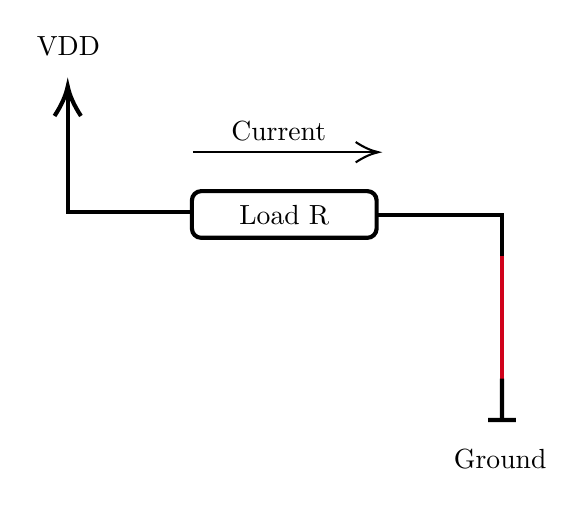
\begin{tikzpicture}[x=0.75pt,y=0.75pt,yscale=-1,xscale=1]
%uncomment if require: \path (0,240); %set diagram left start at 0, and has height of 240

%Straight Lines [id:da008984438739192413] 
\draw [color={rgb, 255:red, 0; green, 0; blue, 0 }  ,draw opacity=1 ][line width=1.5]    (91,99) -- (31.67,99) -- (31.67,41.33) ;
\draw [shift={(31.67,38.33)}, rotate = 450] [color={rgb, 255:red, 0; green, 0; blue, 0 }  ,draw opacity=1 ][line width=1.5]    (14.21,-6.37) .. controls (9.04,-2.99) and (4.3,-0.87) .. (0,0) .. controls (4.3,0.87) and (9.04,2.99) .. (14.21,6.37)   ;

%Rounded Rect [id:dp7662687261949606] 
\draw  [line width=1.5]  (91.5,93.25) .. controls (91.5,90.76) and (93.51,88.75) .. (96,88.75) -- (176,88.75) .. controls (178.49,88.75) and (180.5,90.76) .. (180.5,93.25) -- (180.5,106.75) .. controls (180.5,109.24) and (178.49,111.25) .. (176,111.25) -- (96,111.25) .. controls (93.51,111.25) and (91.5,109.24) .. (91.5,106.75) -- cycle ;
%Straight Lines [id:da19872085195301215] 
\draw [line width=1.5]    (181,100.25) -- (240.75,100.25) -- (240.75,120.13) ;


%Straight Lines [id:da8624965983535746] 
\draw [color={rgb, 255:red, 208; green, 2; blue, 27 }  ,draw opacity=1 ][line width=1.5]    (240.88,120.13) -- (240.88,179.13) ;


%Straight Lines [id:da9869704930235617] 
\draw [line width=1.5]    (240.88,179.13) -- (240.9,199) ;
\draw [shift={(240.9,199)}, rotate = 269.93] [color={rgb, 255:red, 0; green, 0; blue, 0 }  ][line width=1.5]    (0,6.71) -- (0,-6.71)   ;

%Straight Lines [id:da3727804380230437] 
\draw [line width=0.75]    (92,70) -- (179.33,70) ;
\draw [shift={(181.33,70)}, rotate = 180] [color={rgb, 255:red, 0; green, 0; blue, 0 }  ][line width=0.75]    (10.93,-4.9) .. controls (6.95,-2.3) and (3.31,-0.67) .. (0,0) .. controls (3.31,0.67) and (6.95,2.3) .. (10.93,4.9)   ;


% Text Node
\draw (136,100) node [scale=1] [align=left] {Load R};
% Text Node
\draw (133.33,59.67) node  [align=left] {Current};
% Text Node
\draw (240,218) node  [align=left] {Ground};
% Text Node
\draw (32,19) node  [align=left] {VDD};


\end{tikzpicture}
    \caption{short(low resistance) circuit between the load and the ground.} \label{fig:circuit1}
\end{figure}

If we connect an open circuit after the load (See Figure \ref{fig:circuit2}), it
will increase the resistance to a very high value, causing the current to become
effectively zero. And if the current is zero - the voltage is also zero (Ohm's
Law).

\begin{figure}[!ht]
    \centering
    

\tikzset{every picture/.style={line width=0.75pt}} %set default line width to 0.75pt        

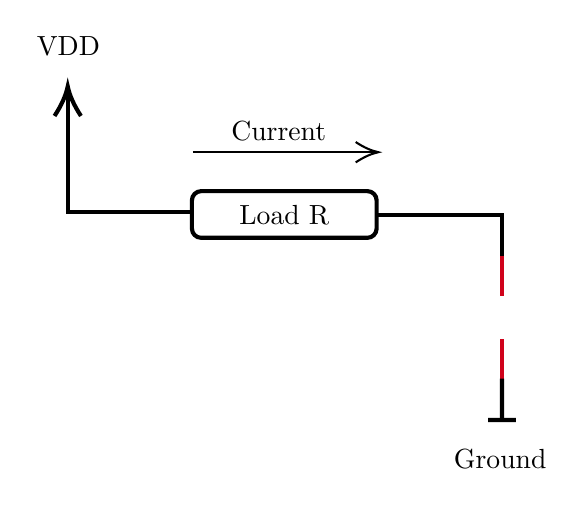
\begin{tikzpicture}[x=0.75pt,y=0.75pt,yscale=-1,xscale=1]
%uncomment if require: \path (0,240); %set diagram left start at 0, and has height of 240

%Straight Lines [id:da008984438739192413] 
\draw [color={rgb, 255:red, 0; green, 0; blue, 0 }  ,draw opacity=1 ][line width=1.5]    (91,99) -- (31.67,99) -- (31.67,41.33) ;
\draw [shift={(31.67,38.33)}, rotate = 450] [color={rgb, 255:red, 0; green, 0; blue, 0 }  ,draw opacity=1 ][line width=1.5]    (14.21,-6.37) .. controls (9.04,-2.99) and (4.3,-0.87) .. (0,0) .. controls (4.3,0.87) and (9.04,2.99) .. (14.21,6.37)   ;

%Rounded Rect [id:dp7662687261949606] 
\draw  [line width=1.5]  (91.5,93.25) .. controls (91.5,90.76) and (93.51,88.75) .. (96,88.75) -- (176,88.75) .. controls (178.49,88.75) and (180.5,90.76) .. (180.5,93.25) -- (180.5,106.75) .. controls (180.5,109.24) and (178.49,111.25) .. (176,111.25) -- (96,111.25) .. controls (93.51,111.25) and (91.5,109.24) .. (91.5,106.75) -- cycle ;
%Straight Lines [id:da19872085195301215] 
\draw [line width=1.5]    (181,100.25) -- (240.75,100.25) -- (240.75,120.13) ;


%Straight Lines [id:da8624965983535746] 
\draw [color={rgb, 255:red, 208; green, 2; blue, 27 }  ,draw opacity=1 ][line width=1.5]    (240.88,160) -- (240.88,179.13) ;


%Straight Lines [id:da9869704930235617] 
\draw [line width=1.5]    (240.88,179.13) -- (240.9,199) ;
\draw [shift={(240.9,199)}, rotate = 269.93] [color={rgb, 255:red, 0; green, 0; blue, 0 }  ][line width=1.5]    (0,6.71) -- (0,-6.71)   ;

%Straight Lines [id:da3727804380230437] 
\draw [line width=0.75]    (92,70) -- (179.33,70) ;
\draw [shift={(181.33,70)}, rotate = 180] [color={rgb, 255:red, 0; green, 0; blue, 0 }  ][line width=0.75]    (10.93,-4.9) .. controls (6.95,-2.3) and (3.31,-0.67) .. (0,0) .. controls (3.31,0.67) and (6.95,2.3) .. (10.93,4.9)   ;

%Straight Lines [id:da775249144810833] 
\draw [color={rgb, 255:red, 208; green, 2; blue, 27 }  ,draw opacity=1 ][line width=1.5]    (240.75,120.13) -- (240.75,139.25) ;



% Text Node
\draw (136,100) node [scale=1] [align=left] {Load R};
% Text Node
\draw (133.33,59.67) node  [align=left] {Current};
% Text Node
\draw (240,218) node  [align=left] {Ground};
% Text Node
\draw (32,19) node  [align=left] {VDD};


\end{tikzpicture}

    \caption{open circuit after the load.} \label{fig:circuit2}
\end{figure}

\subsubsection{Connecting in parallel}

If we connect an open circuit in parallel to the load (See Figure
\ref{fig:circuit3}), the current will flow only through the load's path, so the
current on the open circuit will be 0. However, the voltage drop between both
points of the open circuit will be the same as the drop between the load sides.

\begin{figure}[!ht]
    \centering
    

\tikzset{every picture/.style={line width=0.75pt}} %set default line width to 0.75pt        

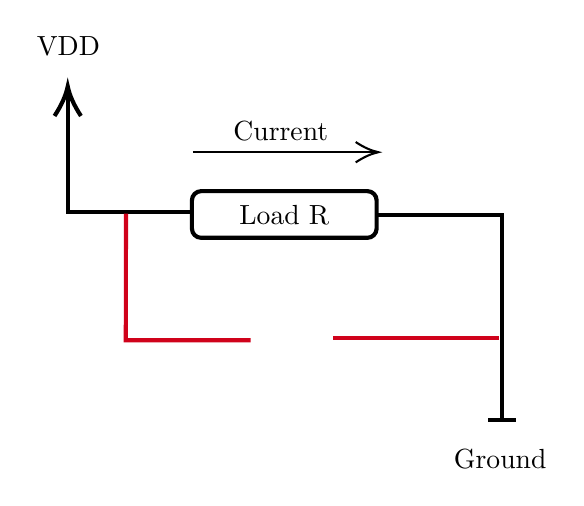
\begin{tikzpicture}[x=0.75pt,y=0.75pt,yscale=-1,xscale=1]
%uncomment if require: \path (0,250); %set diagram left start at 0, and has height of 250

%Straight Lines [id:da008984438739192413] 
\draw [color={rgb, 255:red, 0; green, 0; blue, 0 }  ,draw opacity=1 ][line width=1.5]    (91,99) -- (31.67,99) -- (31.67,41.33) ;
\draw [shift={(31.67,38.33)}, rotate = 450] [color={rgb, 255:red, 0; green, 0; blue, 0 }  ,draw opacity=1 ][line width=1.5]    (14.21,-6.37) .. controls (9.04,-2.99) and (4.3,-0.87) .. (0,0) .. controls (4.3,0.87) and (9.04,2.99) .. (14.21,6.37)   ;

%Rounded Rect [id:dp7662687261949606] 
\draw  [line width=1.5]  (91.5,93.25) .. controls (91.5,90.76) and (93.51,88.75) .. (96,88.75) -- (176,88.75) .. controls (178.49,88.75) and (180.5,90.76) .. (180.5,93.25) -- (180.5,106.75) .. controls (180.5,109.24) and (178.49,111.25) .. (176,111.25) -- (96,111.25) .. controls (93.51,111.25) and (91.5,109.24) .. (91.5,106.75) -- cycle ;
%Straight Lines [id:da19872085195301215] 
\draw [line width=1.5]    (181,100.25) -- (240.75,100.25) -- (240.75,199) ;
\draw [shift={(240.75,199)}, rotate = 270] [color={rgb, 255:red, 0; green, 0; blue, 0 }  ][line width=1.5]    (0,6.71) -- (0,-6.71)   ;

%Straight Lines [id:da3727804380230437] 
\draw [line width=0.75]    (92,70) -- (179.33,70) ;
\draw [shift={(181.33,70)}, rotate = 180] [color={rgb, 255:red, 0; green, 0; blue, 0 }  ][line width=0.75]    (10.93,-4.9) .. controls (6.95,-2.3) and (3.31,-0.67) .. (0,0) .. controls (3.31,0.67) and (6.95,2.3) .. (10.93,4.9)   ;

%Straight Lines [id:da4889722354710415] 
\draw [color={rgb, 255:red, 208; green, 2; blue, 27 }  ,draw opacity=1 ][line width=1.5]    (59.73,99.6) -- (59.65,160.6) -- (119.75,160.6) ;


%Straight Lines [id:da969741666977372] 
\draw [color={rgb, 255:red, 208; green, 2; blue, 27 }  ,draw opacity=1 ][line width=1.5]    (159.5,159.67) -- (239.25,159.67) ;



% Text Node
\draw (136,100) node [scale=1] [align=left] {Load R};
% Text Node
\draw (134.33,59.67) node  [align=left] {Current};
% Text Node
\draw (240,218) node  [align=left] {Ground};
% Text Node
\draw (32,19) node  [align=left] {VDD};


\end{tikzpicture}
    \caption{A close circuit in parallel to the load.} \label{fig:circuit3}
\end{figure}

If we connect a short circuit in parallel to the load (See Figure
\ref{fig:circuit4}), the current will ``prefer" flowing through it rather than
through the load, so the current through the load will be equal to zero, while
the current through the short circuit will be very high - by Ohm's law, since the voltage stays the same as before.

\begin{figure}[!ht]
    \centering
    

\tikzset{every picture/.style={line width=0.75pt}} %set default line width to 0.75pt        

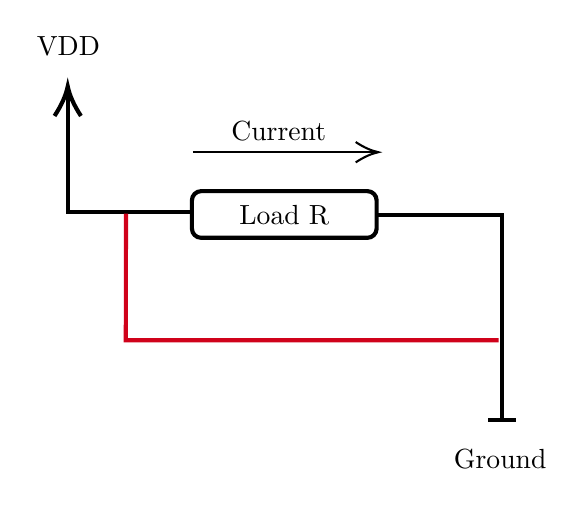
\begin{tikzpicture}[x=0.75pt,y=0.75pt,yscale=-1,xscale=1]
%uncomment if require: \path (0,230.3333282470703); %set diagram left start at 0, and has height of 230.3333282470703

%Straight Lines [id:da008984438739192413] 
\draw [color={rgb, 255:red, 0; green, 0; blue, 0 }  ,draw opacity=1 ][line width=1.5]    (91,99) -- (31.67,99) -- (31.67,41.33) ;
\draw [shift={(31.67,38.33)}, rotate = 450] [color={rgb, 255:red, 0; green, 0; blue, 0 }  ,draw opacity=1 ][line width=1.5]    (14.21,-6.37) .. controls (9.04,-2.99) and (4.3,-0.87) .. (0,0) .. controls (4.3,0.87) and (9.04,2.99) .. (14.21,6.37)   ;

%Rounded Rect [id:dp7662687261949606] 
\draw  [line width=1.5]  (91.5,93.25) .. controls (91.5,90.76) and (93.51,88.75) .. (96,88.75) -- (176,88.75) .. controls (178.49,88.75) and (180.5,90.76) .. (180.5,93.25) -- (180.5,106.75) .. controls (180.5,109.24) and (178.49,111.25) .. (176,111.25) -- (96,111.25) .. controls (93.51,111.25) and (91.5,109.24) .. (91.5,106.75) -- cycle ;
%Straight Lines [id:da19872085195301215] 
\draw [line width=1.5]    (181,100.25) -- (240.75,100.25) -- (240.75,199) ;
\draw [shift={(240.75,199)}, rotate = 270] [color={rgb, 255:red, 0; green, 0; blue, 0 }  ][line width=1.5]    (0,6.71) -- (0,-6.71)   ;

%Straight Lines [id:da3727804380230437] 
\draw [line width=0.75]    (92,70) -- (179.33,70) ;
\draw [shift={(181.33,70)}, rotate = 180] [color={rgb, 255:red, 0; green, 0; blue, 0 }  ][line width=0.75]    (10.93,-4.9) .. controls (6.95,-2.3) and (3.31,-0.67) .. (0,0) .. controls (3.31,0.67) and (6.95,2.3) .. (10.93,4.9)   ;

%Straight Lines [id:da4889722354710415] 
\draw [color={rgb, 255:red, 208; green, 2; blue, 27 }  ,draw opacity=1 ][line width=1.5]    (59.73,99.6) -- (59.65,160.6) -- (239.33,160.6) ;



% Text Node
\draw (136,100) node [scale=1] [align=left] {Load R};
% Text Node
\draw (133.33,59.67) node  [align=left] {Current};
% Text Node
\draw (240,218) node  [align=left] {Ground};
% Text Node
\draw (32,19) node  [align=left] {VDD};


\end{tikzpicture}
    \caption{A short circuit in parallel to the load.} \label{fig:circuit4}
\end{figure}

Since the cable is not a perfect conductor, some of the energy will be consumed
in the form of thermal work, so the cable will heat up.

\section{Measuring Power Consumption}

As an attacker, we want to measure the power consumption of the load in order to deduce interesting insights about it.
For this, we are going to use an Amperemeter.

\subsection{Amperemeter}

An Amperemeter is a device capable of measuring the amount of electric current going through it. It has a very low resistance, so it doesn't affect the circuit it connects to - since it is basically equivalent to an extra piece of conducting wire.

\begin{figure}[!ht]
    \centering
    

\tikzset{every picture/.style={line width=0.75pt}} %set default line width to 0.75pt        

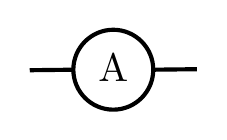
\begin{tikzpicture}[x=0.75pt,y=0.75pt,yscale=-1,xscale=1]
%uncomment if require: \path (0,80.33332824707031); %set diagram left start at 0, and has height of 80.33332824707031

%Shape: Circle [id:dp8443143357842926] 
\draw  [line width=1.5]  (42,40.58) .. controls (42,29.95) and (50.62,21.33) .. (61.25,21.33) .. controls (71.88,21.33) and (80.5,29.95) .. (80.5,40.58) .. controls (80.5,51.21) and (71.88,59.83) .. (61.25,59.83) .. controls (50.62,59.83) and (42,51.21) .. (42,40.58) -- cycle ;
%Straight Lines [id:da8989689187935987] 
\draw [line width=1.5]    (80.5,40.58) -- (101.5,40.33) ;


%Straight Lines [id:da08094666094700531] 
\draw [line width=1.5]    (21,40.83) -- (42,40.58) ;



% Text Node
\draw (61.25,39.58) node [scale=1.44] [align=left] {A};


\end{tikzpicture}
    \caption{Amperemeter Symbol in Circuit Diagrams.} \label{fig:ampermeter}
\end{figure}

\subsubsection{Using an Amperemeter to measure power consumption}

To use an Amperemeter - we ``cut" the wire connected to the load and connect both sides to the
Amperemeter.(See \Cref{fig:circuit5})

Doing so causes all current flowing through the load to pass through the
Amperemeter as well, so we are able to read the current at any given time.
The resistance of the Amperemeter is very low so it doesn't affect the circuit's voltage.

\begin{figure}[!ht]
    \centering
    

\tikzset{every picture/.style={line width=0.75pt}} %set default line width to 0.75pt        

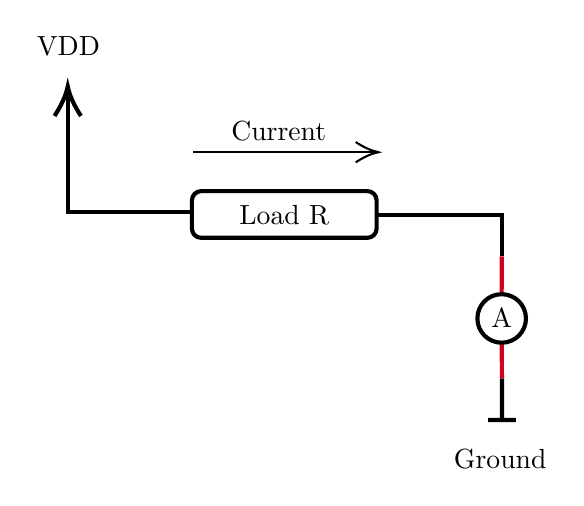
\begin{tikzpicture}[x=0.75pt,y=0.75pt,yscale=-1,xscale=1]
%uncomment if require: \path (0,240); %set diagram left start at 0, and has height of 240

%Straight Lines [id:da008984438739192413] 
\draw [color={rgb, 255:red, 0; green, 0; blue, 0 }  ,draw opacity=1 ][line width=1.5]    (91,99) -- (31.67,99) -- (31.67,41.33) ;
\draw [shift={(31.67,38.33)}, rotate = 450] [color={rgb, 255:red, 0; green, 0; blue, 0 }  ,draw opacity=1 ][line width=1.5]    (14.21,-6.37) .. controls (9.04,-2.99) and (4.3,-0.87) .. (0,0) .. controls (4.3,0.87) and (9.04,2.99) .. (14.21,6.37)   ;

%Rounded Rect [id:dp7662687261949606] 
\draw  [line width=1.5]  (91.5,93.25) .. controls (91.5,90.76) and (93.51,88.75) .. (96,88.75) -- (176,88.75) .. controls (178.49,88.75) and (180.5,90.76) .. (180.5,93.25) -- (180.5,106.75) .. controls (180.5,109.24) and (178.49,111.25) .. (176,111.25) -- (96,111.25) .. controls (93.51,111.25) and (91.5,109.24) .. (91.5,106.75) -- cycle ;
%Straight Lines [id:da19872085195301215] 
\draw [line width=1.5]    (181,100.25) -- (240.75,100.25) -- (240.75,120.13) ;


%Straight Lines [id:da8624965983535746] 
\draw [color={rgb, 255:red, 208; green, 2; blue, 27 }  ,draw opacity=1 ][line width=1.5]    (240.74,161.79) -- (240.88,179.13) ;


%Straight Lines [id:da9869704930235617] 
\draw [line width=1.5]    (240.88,179.13) -- (240.9,199) ;
\draw [shift={(240.9,199)}, rotate = 269.93] [color={rgb, 255:red, 0; green, 0; blue, 0 }  ][line width=1.5]    (0,6.71) -- (0,-6.71)   ;

%Straight Lines [id:da3727804380230437] 
\draw [line width=0.75]    (92,70) -- (179.33,70) ;
\draw [shift={(181.33,70)}, rotate = 180] [color={rgb, 255:red, 0; green, 0; blue, 0 }  ][line width=0.75]    (10.93,-4.9) .. controls (6.95,-2.3) and (3.31,-0.67) .. (0,0) .. controls (3.31,0.67) and (6.95,2.3) .. (10.93,4.9)   ;

%Straight Lines [id:da775249144810833] 
\draw [color={rgb, 255:red, 208; green, 2; blue, 27 }  ,draw opacity=1 ][line width=1.5]    (240.75,120.13) -- (240.74,138.4) ;


%Shape: Circle [id:dp5127141465445768] 
\draw  [line width=1.5]  (229.04,150.09) .. controls (229.04,143.63) and (234.28,138.4) .. (240.74,138.4) .. controls (247.2,138.4) and (252.44,143.63) .. (252.44,150.09) .. controls (252.44,156.55) and (247.2,161.79) .. (240.74,161.79) .. controls (234.28,161.79) and (229.04,156.55) .. (229.04,150.09) -- cycle ;

% Text Node
\draw (136,100) node [scale=1] [align=left] {Load R};
% Text Node
\draw (133.33,59.67) node  [align=left] {Current};
% Text Node
\draw (240,218) node  [align=left] {Ground};
% Text Node
\draw (32,19) node  [align=left] {VDD};
% Text Node
\draw (240.74,150.09) node  [align=left] {A};


\end{tikzpicture}
    \caption{an Amperemeter connected in serial.} \label{fig:circuit5}
\end{figure}

To measure the power consumption, we measure the current ($I$) and since the voltage ($V$) 
hasn't changed, we can compute the power consumption as $P=I \cdot V$.
One major shortcoming of this method is that sometimes we don't want (or can't) 
cut the circuit to connect an Amperemeter. A potential alternative would be to connect the Amperemeter in parallel (See \Cref{fig:circuit6})

\begin{figure}[!ht]
    \centering
    

\tikzset{every picture/.style={line width=0.75pt}} %set default line width to 0.75pt        

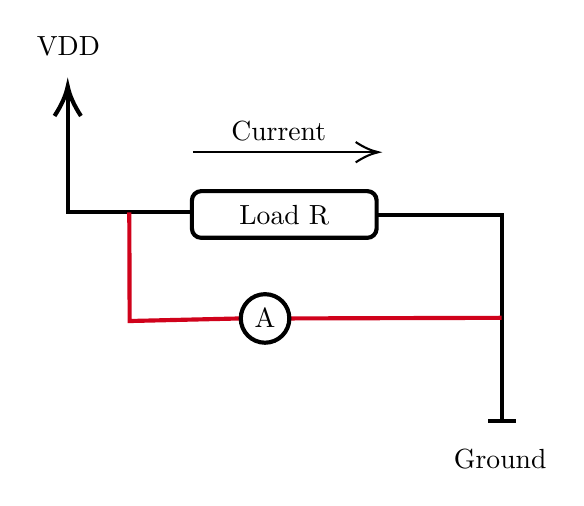
\begin{tikzpicture}[x=0.75pt,y=0.75pt,yscale=-1,xscale=1]
%uncomment if require: \path (0,240); %set diagram left start at 0, and has height of 240

%Straight Lines [id:da008984438739192413] 
\draw [color={rgb, 255:red, 0; green, 0; blue, 0 }  ,draw opacity=1 ][line width=1.5]    (91,99) -- (31.67,99) -- (31.67,41.33) ;
\draw [shift={(31.67,38.33)}, rotate = 450] [color={rgb, 255:red, 0; green, 0; blue, 0 }  ,draw opacity=1 ][line width=1.5]    (14.21,-6.37) .. controls (9.04,-2.99) and (4.3,-0.87) .. (0,0) .. controls (4.3,0.87) and (9.04,2.99) .. (14.21,6.37)   ;

%Rounded Rect [id:dp7662687261949606] 
\draw  [line width=1.5]  (91.5,93.25) .. controls (91.5,90.76) and (93.51,88.75) .. (96,88.75) -- (176,88.75) .. controls (178.49,88.75) and (180.5,90.76) .. (180.5,93.25) -- (180.5,106.75) .. controls (180.5,109.24) and (178.49,111.25) .. (176,111.25) -- (96,111.25) .. controls (93.51,111.25) and (91.5,109.24) .. (91.5,106.75) -- cycle ;
%Straight Lines [id:da19872085195301215] 
\draw [line width=1.5]    (181,100.25) -- (240.75,100.25) -- (240.75,199.33) ;
\draw [shift={(240.75,199.33)}, rotate = 270] [color={rgb, 255:red, 0; green, 0; blue, 0 }  ][line width=1.5]    (0,6.71) -- (0,-6.71)   ;

%Straight Lines [id:da8624965983535746] 
\draw [color={rgb, 255:red, 208; green, 2; blue, 27 }  ,draw opacity=1 ][line width=1.5]    (138.44,150.09) -- (240.75,149.79) ;


%Straight Lines [id:da3727804380230437] 
\draw [line width=0.75]    (92,70) -- (179.33,70) ;
\draw [shift={(181.33,70)}, rotate = 180] [color={rgb, 255:red, 0; green, 0; blue, 0 }  ][line width=0.75]    (10.93,-4.9) .. controls (6.95,-2.3) and (3.31,-0.67) .. (0,0) .. controls (3.31,0.67) and (6.95,2.3) .. (10.93,4.9)   ;

%Straight Lines [id:da775249144810833] 
\draw [color={rgb, 255:red, 208; green, 2; blue, 27 }  ,draw opacity=1 ][line width=1.5]    (61.33,99) -- (61.5,151.33) -- (115.04,150.09) ;


%Shape: Circle [id:dp5127141465445768] 
\draw  [line width=1.5]  (115.04,150.09) .. controls (115.04,143.63) and (120.28,138.4) .. (126.74,138.4) .. controls (133.2,138.4) and (138.44,143.63) .. (138.44,150.09) .. controls (138.44,156.55) and (133.2,161.79) .. (126.74,161.79) .. controls (120.28,161.79) and (115.04,156.55) .. (115.04,150.09) -- cycle ;

% Text Node
\draw (136,100) node [scale=1] [align=left] {Load R};
% Text Node
\draw (133.33,59.67) node  [align=left] {Current};
% Text Node
\draw (240,218) node  [align=left] {Ground};
% Text Node
\draw (32,19) node  [align=left] {VDD};
% Text Node
\draw (126.74,150.09) node  [align=left] {A};


\end{tikzpicture}
    \caption{An Amperemeter connected in parallel to the load} \label{fig:circuit6}
\end{figure}

However, connecting the Amperemeter in parallel would actually burn the Amperemeter as it has no resistance and so, all of the current will flow through it. So, instead of an
Amperemeter we can use a Voltmeter as in  \Cref{fig:circuit7}.

\subsection{Voltmeter}

\begin{figure}[!ht]
    \centering
    

\tikzset{every picture/.style={line width=0.75pt}} %set default line width to 0.75pt        

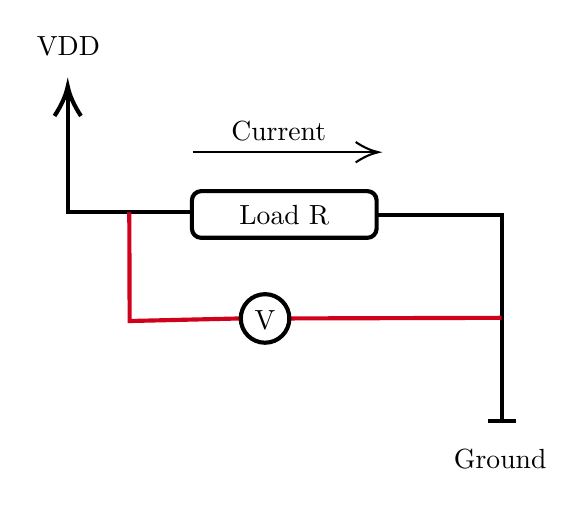
\begin{tikzpicture}[x=0.75pt,y=0.75pt,yscale=-1,xscale=1]
%uncomment if require: \path (0,240); %set diagram left start at 0, and has height of 240

%Straight Lines [id:da008984438739192413] 
\draw [color={rgb, 255:red, 0; green, 0; blue, 0 }  ,draw opacity=1 ][line width=1.5]    (91,99) -- (31.67,99) -- (31.67,41.33) ;
\draw [shift={(31.67,38.33)}, rotate = 450] [color={rgb, 255:red, 0; green, 0; blue, 0 }  ,draw opacity=1 ][line width=1.5]    (14.21,-6.37) .. controls (9.04,-2.99) and (4.3,-0.87) .. (0,0) .. controls (4.3,0.87) and (9.04,2.99) .. (14.21,6.37)   ;

%Rounded Rect [id:dp7662687261949606] 
\draw  [line width=1.5]  (91.5,93.25) .. controls (91.5,90.76) and (93.51,88.75) .. (96,88.75) -- (176,88.75) .. controls (178.49,88.75) and (180.5,90.76) .. (180.5,93.25) -- (180.5,106.75) .. controls (180.5,109.24) and (178.49,111.25) .. (176,111.25) -- (96,111.25) .. controls (93.51,111.25) and (91.5,109.24) .. (91.5,106.75) -- cycle ;
%Straight Lines [id:da19872085195301215] 
\draw [line width=1.5]    (181,100.25) -- (240.75,100.25) -- (240.75,199.33) ;
\draw [shift={(240.75,199.33)}, rotate = 270] [color={rgb, 255:red, 0; green, 0; blue, 0 }  ][line width=1.5]    (0,6.71) -- (0,-6.71)   ;

%Straight Lines [id:da8624965983535746] 
\draw [color={rgb, 255:red, 208; green, 2; blue, 27 }  ,draw opacity=1 ][line width=1.5]    (138.44,150.09) -- (240.75,149.79) ;


%Straight Lines [id:da3727804380230437] 
\draw [line width=0.75]    (92,70) -- (179.33,70) ;
\draw [shift={(181.33,70)}, rotate = 180] [color={rgb, 255:red, 0; green, 0; blue, 0 }  ][line width=0.75]    (10.93,-4.9) .. controls (6.95,-2.3) and (3.31,-0.67) .. (0,0) .. controls (3.31,0.67) and (6.95,2.3) .. (10.93,4.9)   ;

%Straight Lines [id:da775249144810833] 
\draw [color={rgb, 255:red, 208; green, 2; blue, 27 }  ,draw opacity=1 ][line width=1.5]    (61.33,99) -- (61.5,151.33) -- (115.04,150.09) ;


%Shape: Circle [id:dp5127141465445768] 
\draw  [line width=1.5]  (115.04,150.09) .. controls (115.04,143.63) and (120.28,138.4) .. (126.74,138.4) .. controls (133.2,138.4) and (138.44,143.63) .. (138.44,150.09) .. controls (138.44,156.55) and (133.2,161.79) .. (126.74,161.79) .. controls (120.28,161.79) and (115.04,156.55) .. (115.04,150.09) -- cycle ;

% Text Node
\draw (136,100) node [scale=1] [align=left] {Load R};
% Text Node
\draw (133.33,59.67) node  [align=left] {Current};
% Text Node
\draw (240,218) node  [align=left] {Ground};
% Text Node
\draw (32,19) node  [align=left] {VDD};
% Text Node
\draw (126.74,151.09) node  [align=left] {V};


\end{tikzpicture}
    \caption{a Voltmeter connected in parallel to the load} \label{fig:circuit7}
\end{figure}

The Voltmeter's resistance is very very high so the current will not go through
it. The Voltmeter is measuring the voltage drop between one side of the load and
the other side of it. To measure the current using a Voltmeter we
take a load with a very small resistance and connect it as in \Cref{fig:circuit8}.

\begin{figure}[!ht]
    \centering
    

\tikzset{every picture/.style={line width=0.75pt}} %set default line width to 0.75pt        

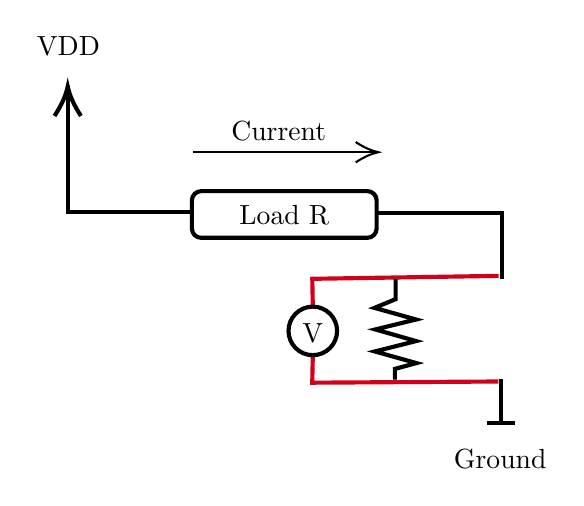
\begin{tikzpicture}[x=0.75pt,y=0.75pt,yscale=-1,xscale=1]
%uncomment if require: \path (0,230.3333282470703); %set diagram left start at 0, and has height of 230.3333282470703

%Straight Lines [id:da008984438739192413] 
\draw [color={rgb, 255:red, 0; green, 0; blue, 0 }  ,draw opacity=1 ][line width=1.5]    (91,99) -- (31.67,99) -- (31.67,41.33) ;
\draw [shift={(31.67,38.33)}, rotate = 450] [color={rgb, 255:red, 0; green, 0; blue, 0 }  ,draw opacity=1 ][line width=1.5]    (14.21,-6.37) .. controls (9.04,-2.99) and (4.3,-0.87) .. (0,0) .. controls (4.3,0.87) and (9.04,2.99) .. (14.21,6.37)   ;

%Rounded Rect [id:dp7662687261949606] 
\draw  [line width=1.5]  (91.5,93.25) .. controls (91.5,90.76) and (93.51,88.75) .. (96,88.75) -- (176,88.75) .. controls (178.49,88.75) and (180.5,90.76) .. (180.5,93.25) -- (180.5,106.75) .. controls (180.5,109.24) and (178.49,111.25) .. (176,111.25) -- (96,111.25) .. controls (93.51,111.25) and (91.5,109.24) .. (91.5,106.75) -- cycle ;
%Straight Lines [id:da19872085195301215] 
\draw [line width=1.5]    (181,99.25) -- (240.75,99.25) -- (240.75,131.08) ;


%Straight Lines [id:da8624965983535746] 
\draw [color={rgb, 255:red, 208; green, 2; blue, 27 }  ,draw opacity=1 ][line width=1.5]    (149.74,144.4) -- (149.5,131) -- (239.25,129.58) ;


%Straight Lines [id:da3727804380230437] 
\draw [line width=0.75]    (92,70) -- (179.33,70) ;
\draw [shift={(181.33,70)}, rotate = 180] [color={rgb, 255:red, 0; green, 0; blue, 0 }  ][line width=0.75]    (10.93,-4.9) .. controls (6.95,-2.3) and (3.31,-0.67) .. (0,0) .. controls (3.31,0.67) and (6.95,2.3) .. (10.93,4.9)   ;

%Straight Lines [id:da775249144810833] 
\draw [color={rgb, 255:red, 208; green, 2; blue, 27 }  ,draw opacity=1 ][line width=1.5]    (149.74,167.79) -- (149.48,181.05) -- (239.19,180.47) ;


%Shape: Circle [id:dp5127141465445768] 
\draw  [line width=1.5]  (138.04,156.09) .. controls (138.04,149.63) and (143.28,144.4) .. (149.74,144.4) .. controls (156.2,144.4) and (161.44,149.63) .. (161.44,156.09) .. controls (161.44,162.55) and (156.2,167.79) .. (149.74,167.79) .. controls (143.28,167.79) and (138.04,162.55) .. (138.04,156.09) -- cycle ;
%Straight Lines [id:da5151277448838241] 
\draw [line width=1.5]    (240.32,179.37) -- (240.32,200.37) ;
\draw [shift={(240.32,200.37)}, rotate = 270] [color={rgb, 255:red, 0; green, 0; blue, 0 }  ][line width=1.5]    (0,6.71) -- (0,-6.71)   ;

%Straight Lines [id:da45585704731206445] 
\draw [line width=1.5]    (189.67,131.2) -- (189.67,140.8) -- (179.47,145) -- (199.47,150.6) -- (179.87,155.4) -- (199.47,161) -- (179.67,166) -- (199.67,171.6) -- (189.27,174.4) -- (189.27,179.6) ;



% Text Node
\draw (136,100) node [scale=1] [align=left] {Load R};
% Text Node
\draw (133.33,59.67) node  [align=left] {Current};
% Text Node
\draw (240,218) node  [align=left] {Ground};
% Text Node
\draw (32,19) node  [align=left] {VDD};
% Text Node
\draw (149.74,157.09) node  [align=left] {V};


\end{tikzpicture}
    \caption{Voltmeter connected in parallel} \label{fig:circuit8}
\end{figure}

By connecting a Voltmeter in parallel with a very small and accurate resistor, we can measure the electric current
using Ohm's law: $I=V/R$
 
\subsection{Power consumption - what's next?}
We saw what power consumption means and how we can measure it. It is very important to
note that for every interesting enough circuit - \textbf{the power consumption varies with time!} 
Our goal, as an attacker, is to find a relationship between the secret information we want to extract and the
power consumption. Then, we can exploit this relationship by measuring the device's/circuit's power consumption 
over time and using this information to extract secret info.

\subsection{Types of electronic components}

Generally speaking, there are two types of components in an electric circuit:
\begin{itemize}
    \item \textbf{Passive devices}: 
    \begin{itemize}
        \item Resistor
        \item Inductor
        \item Capacitor
        \item Diode
    \end{itemize}
    \item \textbf{Active devices}:
    \begin{itemize}
        \item Transistor
        \item Amplifier
        \item Integrated circuit (IC)
    \end{itemize}
\end{itemize}
For us, active devices are much more interesting as their power consumption characteristics change
as a function of the state of the circuit.

\begin{figure}[!ht]
	\centering
	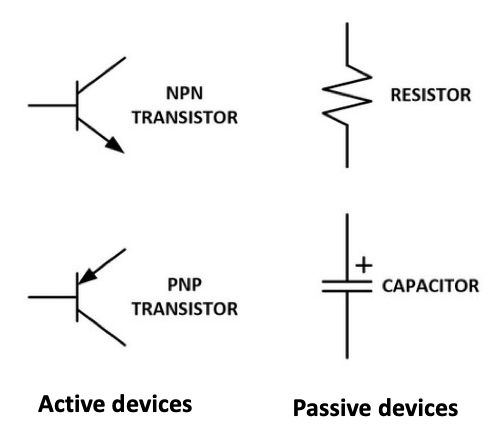
\includegraphics{images/type_of_electronic_components.png}
	\caption{Examples of electronic components.} \label{fig:type_of_electronic_components}
\end{figure}

Specifically, of outmost interest for us is the transistor. 
In integrated circuits, there are lots transistors. Analyzing their power consumption behaiour can
shed a lot of light on the data they're processing,
There are various kinds of transistors and we will concentrate on understanding a
specific type - namely the ``Field-Effect Transistor'' (FET).

\subsection{Field-Effect Transistor}

The Field-Effect Transistor (FET) is an electronic device which uses an electric
field to control the flow of current. FETs are 3-terminalled devices, having a
source, gate, and drain terminals. FETs control the flow of current by the
application of a voltage to the gate terminal, which in turn alters the
conductivity between the drain and source terminals. In order to understand FETs,
we first need to gain some understanding of semiconductors.

\subsection{Semiconductors}

We know that some materials, like copper or gold are good conductors, and others - like plastic or glass are very bad conductors or insulators. 

A \textbf{semi}conductor is a substance, usually a solid chemical element or compound,
that can conduct electricity under some conditions but not others, making it a
good medium for the control of electrical current. Its conductance varies
depending on the current or voltage applied to a control electrode, or on the
intensity of irradiation by infrared (IR), visible light, ultraviolet (UV), or X
rays.

Generally, an atom is built from three sub-particles:
\begin{itemize}
    \item Neutrons - irrelevant for this discussion as they carry no electric charge
    \item Protons - heavy, positively charged particles forming the nucleus of the atom (together with the neutrons).
    \item Electrons - light and negatively charged particles orbiting the atom's nucleus in predefined orbits (this is basically Bohr's model of the atom which isn't quite accurate from the point of view of quantum mechanics, but is a good approximation in our context and in chemistry)
\end{itemize}

The \textbf{Silicon} atom has four electrons in its outer orbit (also known as \textit{valence electrons}).
In Silicon crystals, all of those outer orbit electrons are involved in the covalent bonds between the Silicon atoms.
This implies that pure Silicon is a pretty bad conductor, 
since conductance relies on the flow of free electros,
which are very hard to find in Silicon crystals as all outer-orbit electrons are busy forming covalent bonds and aren't free to move around between atoms.

We can change the behavior of the silicon and turn it into a conductor by doping it - i.e. mixing a small amount of an impurity into the silicon crystal.

There are two types of such useful impurities we can introduce:
\begin{itemize}
    \item N-type – where phosphorus or arsenic is added to the silicon in small
    quantities. They both have five outer orbit electrons, so one of them is out of
    place when they get into the silicon lattice. While having nothing to bond
    to, the fifth electron is free to move around. As electrons have a negative
    charge, this kind of impurity is called N-type (N = Negative).
    \item P-type - where boron or gallium is added to the silicon. They both
    have only three outer electrons. So, when we mix them into the silicon
    lattice, there will be ``holes" in the lattice where a silicon electron has
    nothing to bond to. The hole is looking for an electron from a neighbor atom
    and when that happens the hole is ``moving". As the absence of an electron
    creates the effect of a positive charge, this kind of impurity is called
    P-type (P = Positive).
\end{itemize}

\subsection{How does the Field-Effect Transistor work? }

\begin{figure}[!ht]
	\centering
	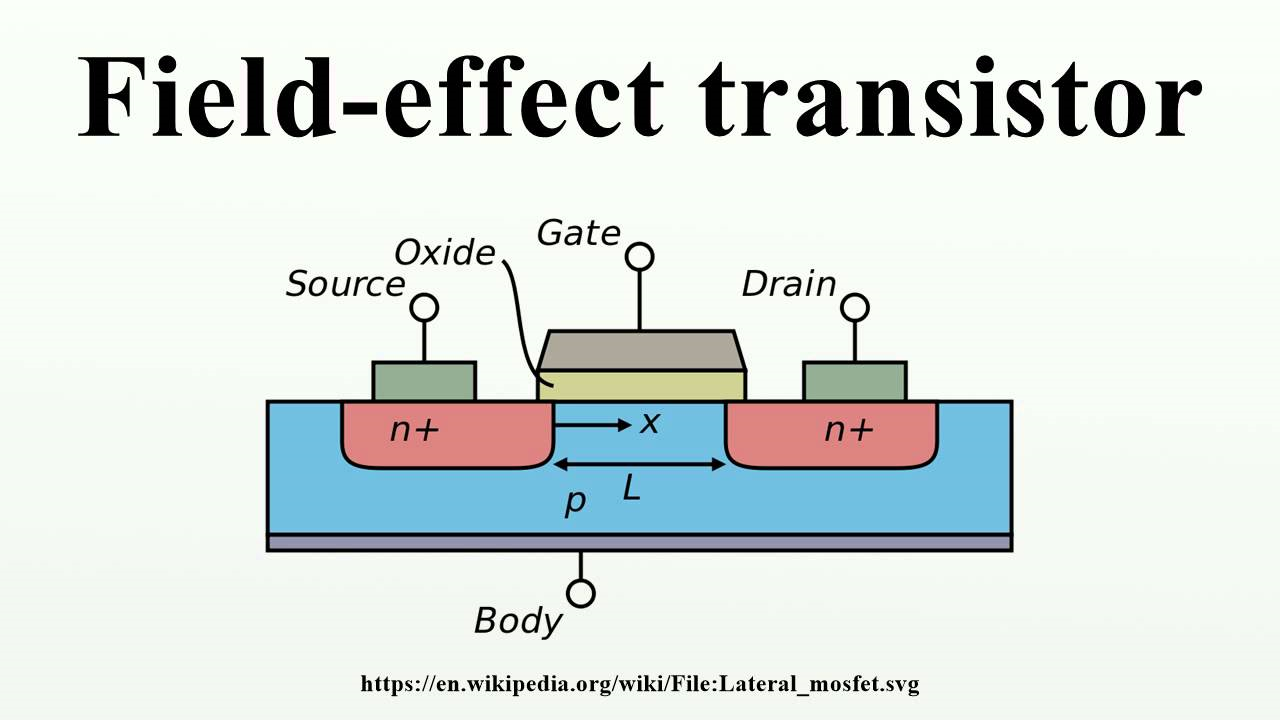
\includegraphics{images/field_effect_transistor.png}
	\caption{Field-Effect Transistor.} \label{fig:field_effect_transistor}
\end{figure}

In the Field-Effect Transistor there are two ``n+" areas with N-type doping and a ``p" area with P-type doping (see \Cref{fig:field_effect_transistor}). The
``n+" areas contain a lot of free electrons and the ``p" area contains a lot of
``holes". Initially, the free electrons from the ``n+" areas are moving into the holes in the ``p'' area and the transistor as a whole is not conducting  any current form the Source to the Drain (i.e. is an open circuit) as there are no free electrons that can move around. When an electrical field is applied to the Gate it gets charged with lots of free electrons. These electrons in the Gate can't move to the Silicon itself as there is an insulating oxide layer between them, but the repulsive force between the negatively charged electrons pushes the electrons in the part of the ``p"" area between the ``n+" areas to the bottom creating a ``channel" allowing the flow of electrons from Source to the Drain through the holes left by the electrons the were pushed away - thus turning the transistor into a conductor (i.e. closed/short circuit).

\subsection{Buliding an Amplifier using a FET}
We can easily construct an Amplifier using a FET by connecting the input signal to the FET's Gate terminal and the power supply to the Source terminal. Then, the Drain terminal's output current will be an amplification of the input signal going into the Gate.

\subsection{CMOS}
Complementary Metal Oxide Semiconductor (CMOS) is a method for creating logical gates. Its core concept is based on using a ``pull up network'' (Vdd) denoting a logical 1 and a ``pull down network'' (Vss) denoting a logical 0. Then, a set of connections and transistors create a closed circuit of either the pull up or the pull down network with the output terminal ``Q'', depending on the value of the input terminal(s). It is very important to design the circuit in such a way that for every input, exactly one of the networks will be close-circuited to the output, since if none of them is close-circuited the output will be undefined and if both of them are close-circuited to the output they will short circuit each other, potentially causing damage to the circuit.

Now, let's see a few examples for implementing logical gates using CMOS.

\subsection{NOT Gate CMOS}

\begin{figure}[!ht]
    \centering
    

\tikzset{every picture/.style={line width=0.75pt}} %set default line width to 0.75pt        

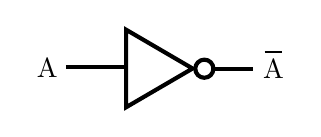
\begin{tikzpicture}[x=0.75pt,y=0.75pt,yscale=-1,xscale=1]
%uncomment if require: \path (0,219); %set diagram left start at 0, and has height of 219

%Straight Lines [id:da07885295239893186] 
\draw [line width=1.5]    (40,39.33) -- (68.5,39.33) ;


%Straight Lines [id:da2596764371394711] 
\draw [line width=1.5]    (110.02,40.17) -- (130.25,40.17) ;

\draw [shift={(106.67,40.17)}, rotate = 0] [color={rgb, 255:red, 0; green, 0; blue, 0 }  ][line width=1.5]      (0, 0) circle [x radius= 4.36, y radius= 4.36]   ;
%Straight Lines [id:da4451475450468101] 
\draw [line width=0.75]    (135.67,32.17) -- (144,32.17) ;


%Flowchart: Extract [id:dp4235554887602122] 
\draw  [line width=1.5]  (101,40.07) -- (69,58.73) -- (69,21.4) -- cycle ;

% Text Node
\draw (31,40) node  [align=left] {A};
% Text Node
\draw (140,40.5) node  [align=left] {A};


\end{tikzpicture}
    \caption{Logical NOT Gate} \label{fig:not}
\end{figure}


\begin{figure}[!ht]
    \centering
    

\tikzset{every picture/.style={line width=0.75pt}} %set default line width to 0.75pt        

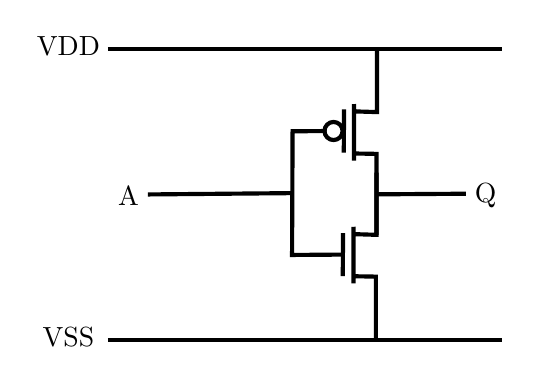
\begin{tikzpicture}[x=0.75pt,y=0.75pt,yscale=-1,xscale=1]
%uncomment if require: \path (0,201.3333282470703); %set diagram left start at 0, and has height of 201.3333282470703

%Straight Lines [id:da07885295239893186] 
\draw [line width=1.5]    (51,30.33) -- (240.75,30.33) ;


%Straight Lines [id:da39856222237487815] 
\draw [line width=1.5]    (180.67,30.67) -- (180.67,60.67) -- (169.71,60.33) -- (169.6,56.8) -- (169.6,84.05) -- (169.6,80.62) -- (180.4,80.8) -- (180.4,119.81) ;


%Straight Lines [id:da5857134524935192] 
\draw [line width=1.5]    (180.4,89.81) -- (180.4,119.81) -- (169.45,119.47) -- (169.33,115.94) -- (169.33,143.19) -- (169.33,139.76) -- (180.13,139.94) -- (180.13,170) ;


%Straight Lines [id:da21313521807196745] 
\draw [line width=1.5]    (51,170.33) -- (240.75,170.33) ;


%Straight Lines [id:da5667092258145612] 
\draw [line width=1.5]    (180.4,100.3) -- (223.5,100) ;


%Straight Lines [id:da6991442899200719] 
\draw [line width=1.5]    (164.67,80.16) -- (164.8,59.4) ;


%Straight Lines [id:da08031166754703278] 
\draw [line width=1.5]    (164.25,129.33) -- (139.75,129.5) -- (140,69.92) -- (156.38,69.8) ;
\draw [shift={(159.73,69.78)}, rotate = 359.6] [color={rgb, 255:red, 0; green, 0; blue, 0 }  ][line width=1.5]      (0, 0) circle [x radius= 4.36, y radius= 4.36]   ;

%Straight Lines [id:da21308267181792218] 
\draw [line width=1.5]    (164.18,139.71) -- (164.32,118.96) ;


%Straight Lines [id:da40299410186396645] 
\draw [line width=1.5]    (70.25,100.35) -- (139.88,99.71) ;



% Text Node
\draw (32,29) node  [align=left] {VDD};
% Text Node
\draw (32,169) node  [align=left] {VSS};
% Text Node
\draw (233,101) node  [align=left] {Q};
% Text Node
\draw (61,101) node  [align=left] {A};


\end{tikzpicture}
    \caption{CMOS NOT gate} \label{fig:circuit9}
\end{figure}

When the voltage of input A is low (A=0), the upper
transistor's channel is closed (since this is a PMOS transistor that closes the circuit when it gets a 0 input signal) and we have a connection between Vdd(1) and Q, so
Q = 1. When the voltage of input A is high (A=1),
the lower transistor's circuit is closed (since it is an NMOS transistor) and we have a connection between Vss(0)
and Q, so Q = 0. It is trivial to see that we've implemented a logical NOT operation with A being the input and Q being the output.

\subsection{When does a CMOS circuit consume power?}

There is an interesting question though – when does this circuit consume power? As mentioned previously, power is consumed when eletric current from the power source (Vdd) reaches the ground (Vss). In our case there is never a connection between Vdd and Vss so it appears power is never consumed, thus defying the energy conservation principcal. The answer to this is that a bit of power is actually consumed when transistors switch between their two possible outputs - i.e. connections with either Vss or Vss. We will see later on, how these minor power consumptions can be used for our purposes.

\begin{table}
    \centering
    \caption{NOT gate truth table.}
    \begin{tabular}{llll}
        \toprule
        \textbf{input}  & A     & 0 & 1 \\ \midrule \textbf{output} & Not A & 1
        & 0 \\ \bottomrule
    \end{tabular}
\end{table} 

\subsection{AND Gate CMOS}

\Cref{fig:and} is a logical AND gate.

\begin{figure}[!ht]
    \centering
    

\tikzset{every picture/.style={line width=0.75pt}} %set default line width to 0.75pt        

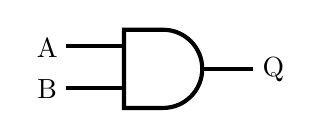
\begin{tikzpicture}[x=0.75pt,y=0.75pt,yscale=-1,xscale=1]
%uncomment if require: \path (0,80.33332824707031); %set diagram left start at 0, and has height of 80.33332824707031

%Straight Lines [id:da07885295239893186] 
\draw [line width=1.5]    (40,29.33) -- (68.5,29.33) ;


%Flowchart: Delay [id:dp4724078764954891] 
\draw  [line width=1.5]  (68,21.33) -- (86.83,21.33) .. controls (97.23,21.33) and (105.67,29.77) .. (105.67,40.17) .. controls (105.67,50.57) and (97.23,59) .. (86.83,59) -- (68,59) -- cycle ;
%Straight Lines [id:da5877789079181] 
\draw [line width=1.5]    (40,49.33) -- (68.5,49.33) ;


%Straight Lines [id:da2596764371394711] 
\draw [line width=1.5]    (106.67,40.17) -- (130.25,40.17) ;



% Text Node
\draw (31,30) node  [align=left] {A};
% Text Node
\draw (31,50) node  [align=left] {B};
% Text Node
\draw (140,40.5) node  [align=left] {Q};


\end{tikzpicture}
    \caption{AND Gate} \label{fig:and}
\end{figure}

We will create a CMOS AND gate using 4 transistors:

\begin{table}[!ht]
    \centering
    \caption{AND gate truth table.}
    \begin{tabular}{lllll}
        \toprule
        \textbf{input a} & 0 & 0 & 1 & 1 \\ \midrule \textbf{input b} & 0 & 1 &
        0 & 1 \\ \midrule \textbf{output}  & 0 & 0 & 0 & 1 \\ \bottomrule
    \end{tabular}
\end{table}

First we want to build the Pull Up Network, so for input A and B, for A=B=1 then
the output Q is 1. Then we will build the Pull Down Network to support the other
combinations of inputs from the truth table to deliver 0 as the output Q.

\subsection{Storage circuits}
Now, let's see how we can use CMOS circuits to store data - i.e. create memory components.
A flip-flop is a circuit, comprised of two latches that has two stable states and can be used to store a single bit of data.
\begin{figure}[!ht]
    \centering
    

\tikzset{every picture/.style={line width=0.75pt}} %set default line width to 0.75pt        

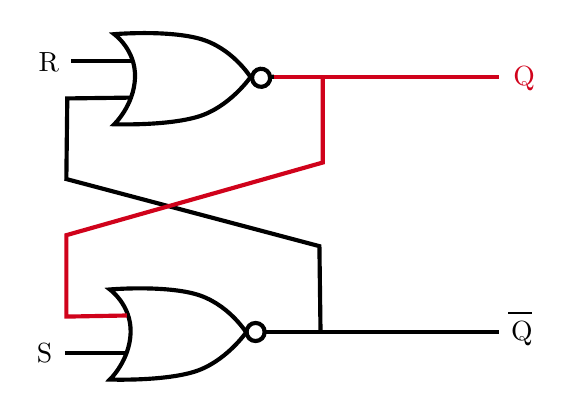
\begin{tikzpicture}[x=0.75pt,y=0.75pt,yscale=-1,xscale=1]
%uncomment if require: \path (0,210.66666412353516); %set diagram left start at 0, and has height of 210.66666412353516

%Shape: Polygon Curved [id:ds6291230594537647] 
\draw  [color={rgb, 255:red, 0; green, 0; blue, 0 }  ,draw opacity=1 ][line width=1.5]  (64.57,15.54) .. controls (64.57,15.54) and (75.02,23.03) .. (74.57,36.44) .. controls (74.11,49.84) and (64.57,58.93) .. (64.57,58.93) .. controls (64.57,58.93) and (89.67,59.83) .. (104.89,55.29) .. controls (120.12,50.74) and (130.23,36.21) .. (130.23,36.21) .. controls (130.23,36.21) and (121.33,21.89) .. (105.43,17.64) .. controls (89.52,13.4) and (64.57,15.54) .. (64.57,15.54) -- cycle ;
%Straight Lines [id:da32731251553352636] 
\draw [color={rgb, 255:red, 0; green, 0; blue, 0 }  ,draw opacity=1 ][line width=1.5]    (43.93,28.6) -- (72.96,28.6) ;


%Straight Lines [id:da3869103872130202] 
\draw [color={rgb, 255:red, 0; green, 0; blue, 0 }  ,draw opacity=1 ][line width=1.5]    (163.94,158.49) -- (163.41,117.67) -- (41.48,85.33) -- (41.94,46.49) -- (72.16,46.1) ;


%Straight Lines [id:da1720618143634285] 
\draw [color={rgb, 255:red, 0; green, 0; blue, 0 }  ,draw opacity=1 ][line width=1.5]    (138.66,36.27) -- (141.5,36.02) ;

\draw [shift={(135.32,36.55)}, rotate = 355.1] [color={rgb, 255:red, 0; green, 0; blue, 0 }  ,draw opacity=1 ][line width=1.5]      (0, 0) circle [x radius= 4.36, y radius= 4.36]   ;
%Straight Lines [id:da9259051839045029] 
\draw [color={rgb, 255:red, 0; green, 0; blue, 0 }  ,draw opacity=1 ][line width=1.5]    (136.02,159.02) -- (250,159.02) ;

\draw [shift={(132.67,159.02)}, rotate = 0] [color={rgb, 255:red, 0; green, 0; blue, 0 }  ,draw opacity=1 ][line width=1.5]      (0, 0) circle [x radius= 4.36, y radius= 4.36]   ;
%Shape: Polygon Curved [id:ds45090218745840094] 
\draw  [color={rgb, 255:red, 0; green, 0; blue, 0 }  ,draw opacity=1 ][line width=1.5]  (62.45,138.53) .. controls (62.45,138.53) and (72.9,146.03) .. (72.45,159.43) .. controls (71.99,172.84) and (62.45,181.93) .. (62.45,181.93) .. controls (62.45,181.93) and (87.55,182.82) .. (102.77,178.28) .. controls (118,173.74) and (128.11,159.21) .. (128.11,159.21) .. controls (128.11,159.21) and (119.21,144.88) .. (103.3,140.64) .. controls (87.4,136.4) and (62.45,138.53) .. (62.45,138.53) -- cycle ;
%Straight Lines [id:da4647074828700599] 
\draw [color={rgb, 255:red, 0; green, 0; blue, 0 }  ,draw opacity=1 ][line width=1.5]    (40.75,169.09) -- (69.78,169.09) ;


%Straight Lines [id:da5333172740033338] 
\draw [color={rgb, 255:red, 208; green, 2; blue, 27 }  ,draw opacity=1 ][line width=1.5]    (165,36.02) -- (165,77.38) -- (41.48,112.37) -- (41.48,151.6) -- (70.64,151.07) ;


%Straight Lines [id:da5430278461164106] 
\draw [color={rgb, 255:red, 208; green, 2; blue, 27 }  ,draw opacity=1 ][line width=1.5]    (141.5,36.02) -- (250,36.02) ;


%Straight Lines [id:da9737841576113742] 
\draw    (254.5,149.67) -- (266,149.67) ;



% Text Node
\draw (33,29) node  [align=left] {R};
% Text Node
\draw (31,169) node  [align=left] {S};
% Text Node
\draw (262,37) node  [align=left] {\textcolor[rgb]{0.82,0.01,0.11}{Q}};
% Text Node
\draw (261,160) node  [align=left] {Q};


\end{tikzpicture}
    \caption{Flipflop} \label{fig:flipflop}
\end{figure}

\begin{figure}[!ht]
	\centering
	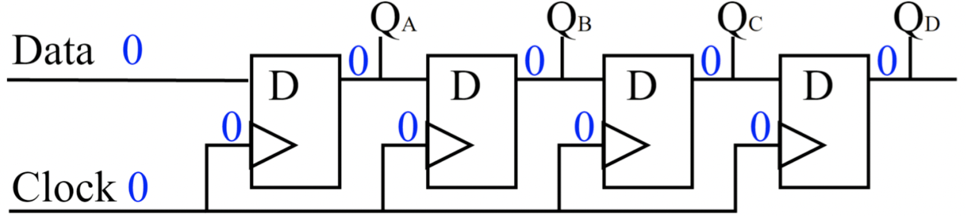
\includegraphics[width=1.0\textwidth]{images/banch_of_flipflops.png}
	\caption{A series of flip-flops} \label{fig:banch_of_flipflops}
\end{figure}

The circuit can be made to change state by signals applied to one or more
control inputs and will have one or two outputs. It is the basic storage element
in sequential logic. Flip-flops and latches are fundamental building blocks of
digital electronics systems used in computers, communications, and many other
types of systems.

A flip-flop is a device which stores a single bit of data; one of
its two states represents a ``one" and the other represents a ``zero". Such data
storage can be used for storage of state, and such a circuit is described as
sequential logic in electronics. When used in a finite-state machine, the output
and next state depend not only on its current input, but also on its current
state (and hence, previous inputs). It can also be used for counting of pulses,
and for synchronizing variably-timed input signals to some reference timing
signal.

Flip-flops can be either level-triggered (asynchronous, transparent or opaque)
or edge-triggered (synchronous, or clocked). The term flip-flop has historically
referred generically to both level-triggered and edge-triggered circuits that
store a single bit of data using gates. We will refer to Flip-Flop as
edge-triggered i.e. clock-synchronized.

It is both interesting and important to note that for each storage element in a circuit
the data/output changes at the same time orchestrated by the clock signal and so we have a combined, amplified signal that we, as attackers, can monitor to extract secret information.

 \subsection {Core i7 chip}
 To demonstrate how combinations of CMOS gates scale up to form real-world chips, \Cref{fig:i7} is an image of a modern Intel core i7 CPU, which is fundamentally a CMOS chip.

\begin{figure}[!ht]
	\centering
	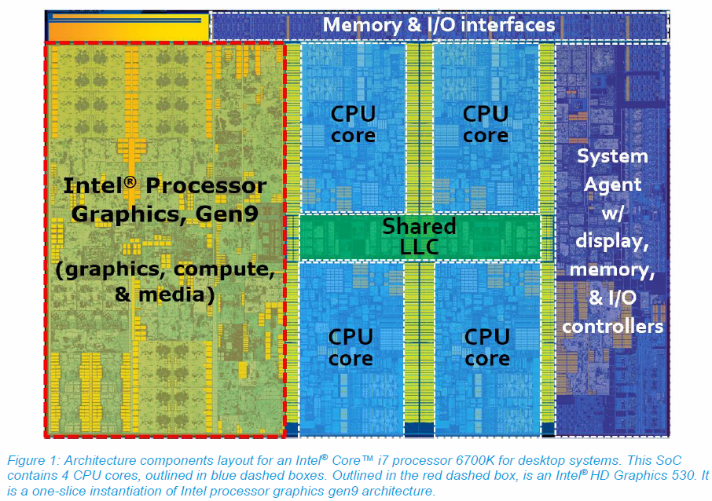
\includegraphics[width=1.0\textwidth]{images/i7.png}
	\caption{Intel i7 CPU} \label{fig:i7}
\end{figure}

We can see a multitude of different components, most notably:
\begin{itemize}
    \item The integrated GPU containing multiple repeating patterns denoting the GPU processing units
    \item The identically looking 4 CPU cores with the repeating yellow patterns of CPU cache memory
\end{itemize}

\subsection {Power Consumption Variability}

\begin{figure}[!ht]
    \centering
    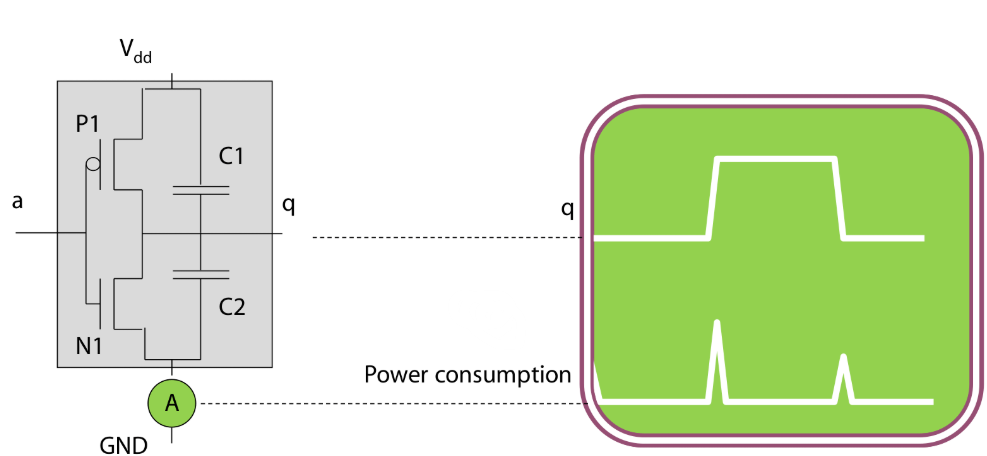
\includegraphics[width=1.0\linewidth]{images/chapter4/not-gate-with-power-consumption-plot.png}
    \caption{Not gate connected to an oscilloscope.} \label{fig:Not gate connected to an oscilloscope}
\end{figure}

In \Cref{fig:Not gate connected to an oscilloscope} we have a CMOS NOT gate, like the one we saw before, with an Amperemeter connected to it to measure the power consumption, and a plot of both the gate's output (q) and power consumption as would've been captured by an oscilloscope connected to the Amperemeter.
C1 and C2 are capacitors that are required due to low-level electrical characteristics which we won't describe in deail.

In the plot we see a few interesting phenomena:
\begin{itemize}
    \item The power consumption is zero when the output (Q) is constant.
    \item There is a spike in power consumption each time the output (Q) changes.
    \item The power consumption spike goes higher when Q changes from 0 to 1 compared to when Q changes from 1 to 0.
\end{itemize}

More generally, power consumption is the sum of the static and the dynamic power
consumption which changes with time: 

\begin{displaymath}
    P(t)=P_{stat} + P_{dyn}(t)
\end{displaymath}

As an attacker, we don't really care about the static power consumption that depends on the device's supply voltage, transistor manufacturing technology, etc.
The dynamic power consumption, on the other hand, depends on the clock rate, the circuit activity and input data. It can reveal a lot about the data flowing through the circuit, which could be very beneficial.

Theoretically, we can accurately measure the full power consumption of the device on the one hand and compute a full power consmuption simulation on the other hand and then try to extract the interesting data by comparing the results and solving the resulting equations to find the data manipulated during the measurement.
However, making this accurate computation isn't feasible and we'll, instead, compromise for an approximate model of the device's power consmuption that will allow us to achive practical results subject to a set of assumptions we'll make about the device.

\subsection {Hamming distance model}
We'll assume the following about the device we wish to attack:
\begin{itemize}
    \item This is a CMOS device.
    \item When it's static in terms of the outputs of its transistors - the static power is very low, and when it switches, there is a relatively high power consumption.
    \item This is synchronous circuit, which means it has a lot of transistors
    that all change at the same time.
    \item The power consumption is proportional to the amount of changes and the
    outputs of these transistors.
\end{itemize}

Count the number of changes in the output bits of the device's transistors brings us to the so called ``Hamming distance model''. 

The \textit{Hamming distance} between two vectors is the number of differing bits between the vectors. 
For example, the Hamming distance between the vectors 01101010 and 11011011 is 4, since they differ in exactly 4 indices, namely: 0,2,3,7.

Formally, assuming we have a vector:
\begin{displaymath}
    X=x_{n},x_{n-1},...,x_{1},x_{0}
\end{displaymath}

We'll first define the ``Hamming weight'' operator:
\begin{displaymath}
    HW(X)=\sum x_{i}
\end{displaymath}

Then, we'll define the ``Hamming distance'': 
\begin{displaymath}
    HD(X,Y)=HW(V_{1} \bigoplus V_{2})
\end{displaymath}

For CMOS devices, we'll approximate the power consumption as proportional to the amount of bit transitions from one to zero or from zero to one - i.e. the hamming distance between the state vectors (the set of all CMOS transistor outputs) of the device across a time interval.

\subsection{Power Consumption Noise}

This is all good in a ``perfectly spherical'' world, but in the real world we still need to account for noise. There are a number different types of noise that affect our power consumption measurements:
\begin{itemize}
    \item \textbf{Switching noise} - computations or some other power consumption occuring in the device except for the computation we want to monitor, that also affect the power consumption. This can be either correlated (i.e. happens every time our target computation is performed) or uncorreleated (i.e. happens in random relative to our target computation and so can be easily reduced by repeating the measurement a few times).
    \item \textbf{Measurement noise} - caused by mild inaccuracies in our measurement equipment and setup.
    \item \textbf{Thermal noise} - noise caused by electrons jumping arround, appearing, disappearing and creating radiation along the way. This noise is higher when the temperature of the device/circuit is higher.
\end{itemize}

To summarize, the actual measured power consumption can be modeled as:
\begin{displaymath}
    P_{meas}(t)=P_{stat} + P_{dyn}(t) + N(t)
\end{displaymath}
(N(t) - Noise)

A number of approaches exist to minimize the amount of noise, depending on its nature:
\begin{itemize}
    \item Repeat the measurement to average out uncorrelated noise.
    \item Control the amount of thermal noise by running the experiment in very low temperatures.
    \item Prevent radiation originating noise by putting the device in a Faraday cage.
    \item Modify the device in a way that either increases the signal or decreases the nosie. For example - remove a noise generating module.
\end{itemize}

Another thing we can do is move from measuring power consumption to measuring electromagnetic radiation.

\subsection {From Power to EM}

\begin{figure}[!ht]
    \centering
    \tikzset{every picture/.style={line width=0.75pt}} %set default line width to 0.75pt        

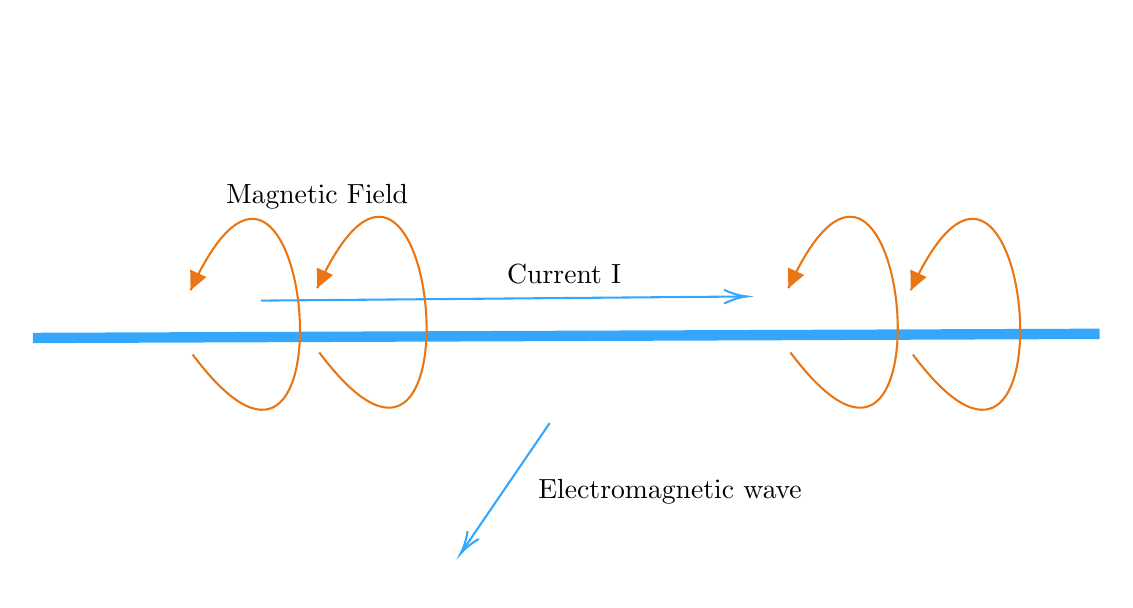
\begin{tikzpicture}[x=0.75pt,y=0.75pt,yscale=-1,xscale=1]
%uncomment if require: \path (0,300); %set diagram left start at 0, and has height of 300

%Straight Lines [id:da730115903310417] 
\draw [color={rgb, 255:red, 52; green, 167; blue, 252 }  ,draw opacity=1 ][line width=3.75]    (69,171) -- (583,169) ;


%Straight Lines [id:da8949672238779289] 
\draw [color={rgb, 255:red, 52; green, 167; blue, 252 }  ,draw opacity=1 ]   (179,153) -- (411,151.02) ;
\draw [shift={(413,151)}, rotate = 539.51] [color={rgb, 255:red, 52; green, 167; blue, 252 }  ,draw opacity=1 ][line width=0.75]    (10.93,-3.29) .. controls (6.95,-1.4) and (3.31,-0.3) .. (0,0) .. controls (3.31,0.3) and (6.95,1.4) .. (10.93,3.29)   ;

%Curve Lines [id:da4084322101826783] 
\draw [color={rgb, 255:red, 233; green, 117; blue, 20 }  ,draw opacity=1 ]   (493,179) .. controls (574,287) and (549,23) .. (492,148) ;
\draw [shift={(492,148)}, rotate = 294.51] [fill={rgb, 255:red, 233; green, 117; blue, 20 }  ,fill opacity=1 ][line width=0.75]  [draw opacity=0] (8.93,-4.29) -- (0,0) -- (8.93,4.29) -- cycle    ;

%Straight Lines [id:da8207423009134964] 
\draw [color={rgb, 255:red, 52; green, 167; blue, 252 }  ,draw opacity=1 ]   (318,212) -- (276.13,273.35) ;
\draw [shift={(275,275)}, rotate = 304.32] [color={rgb, 255:red, 52; green, 167; blue, 252 }  ,draw opacity=1 ][line width=0.75]    (10.93,-3.29) .. controls (6.95,-1.4) and (3.31,-0.3) .. (0,0) .. controls (3.31,0.3) and (6.95,1.4) .. (10.93,3.29)   ;

%Curve Lines [id:da43215348815507637] 
\draw [color={rgb, 255:red, 233; green, 117; blue, 20 }  ,draw opacity=1 ]   (434,178) .. controls (515,286) and (490,22) .. (433,147) ;
\draw [shift={(433,147)}, rotate = 294.51] [fill={rgb, 255:red, 233; green, 117; blue, 20 }  ,fill opacity=1 ][line width=0.75]  [draw opacity=0] (8.93,-4.29) -- (0,0) -- (8.93,4.29) -- cycle    ;

%Curve Lines [id:da7658292921428724] 
\draw [color={rgb, 255:red, 233; green, 117; blue, 20 }  ,draw opacity=1 ]   (146,179) .. controls (227,287) and (202,23) .. (145,148) ;
\draw [shift={(145,148)}, rotate = 294.51] [fill={rgb, 255:red, 233; green, 117; blue, 20 }  ,fill opacity=1 ][line width=0.75]  [draw opacity=0] (8.93,-4.29) -- (0,0) -- (8.93,4.29) -- cycle    ;

%Curve Lines [id:da6169102709245924] 
\draw [color={rgb, 255:red, 233; green, 117; blue, 20 }  ,draw opacity=1 ]   (207,178) .. controls (288,286) and (263,22) .. (206,147) ;
\draw [shift={(206,147)}, rotate = 294.51] [fill={rgb, 255:red, 233; green, 117; blue, 20 }  ,fill opacity=1 ][line width=0.75]  [draw opacity=0] (8.93,-4.29) -- (0,0) -- (8.93,4.29) -- cycle    ;


% Text Node
\draw (206,103) node  [align=left] {Magnetic Field};
% Text Node
\draw (325,140) node  [align=left] {Current I};
% Text Node
\draw (376,245) node  [align=left] {Electromagnetic wave};


\end{tikzpicture}


    \caption{electromagnetic emission.} \label{fig:electromagnetic emission}
\end{figure}

A fundamental law of physics states that moving charged particles create magnetic fields. Specifically, a directed electric current creates a magnetic field with magnitude and orientation descibred by the Biot-Savart law. The direction of the magnetic field can be found using the ``left hand rule'' (\Cref{fig:electromagnetic emission}). This is very good news for us, as this means that instead of measuring the power consumption, we can simply measure the magnetic field and from it deduce the magnitude of the electric current that is its source.
One disadvantage of this method is that it is very localized, so we need to get VERY close to the device or alternatively point a very sensitive directional antenna to it to make measurements.

\subsection{Measurement setups}
We'll now take a look at a few examples of attacker setups.

\subsubsection{Power measurement setup}

\begin{figure}[!ht]
    \centering
    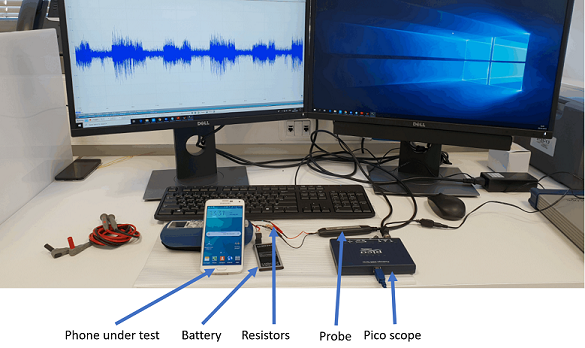
\includegraphics[width=1.0\linewidth]{images/chapter4/power_measurement_setup.png}
    \caption{Power measurement setup} \label{fig:power_measurement_setup}
\end{figure}

In \Cref{fig:power_measurement_setup} we have:
\begin{itemize}
    \item A Pico scope - a small oscilloscope that measures voltage over time.
    \item A Voltmeter probe that is connected to the battery of the phone under test using a bunch of small resistors connected in parallel - this is a way to measure the current, as we explained above.
\end{itemize}

\subsubsection{EM measurement setup}
\begin{figure}[!ht]
    \centering
    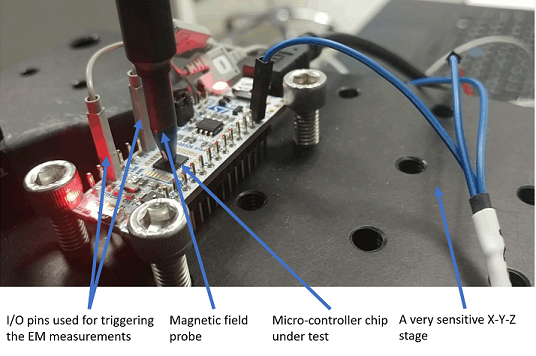
\includegraphics[width=1.0\linewidth]{images/chapter4/em_measurement_setup.png}
    \caption{EM measurement setup} \label{fig:em_measurement_setup}
\end{figure}

In \Cref{fig:em_measurement_setup} we want to measure the EM field of a micro controller chip. We place the whole setup on a computer-controlled XYZ stage that allow placing the board very close to the Magnetic field probe with very high (micron level) precision - this is crucial since electromagnetic emanations can only be recorded from a very close distance. Another important thing to note is the pair of gray cables connected to I/O pins on the board, used for triggering the beginning and end of the measurement - this is very beneficial because it allows us to accuretly measure the EM field for a very short time interval during which the computations we'd like to track occur. A short time interval allows us recording with a higher resolution, gaining more valuable info that will help analyse the signal to extract the secret data we want.

\subsubsection{Generic attack setup schematic}
\begin{figure}[!ht]
    \centering
    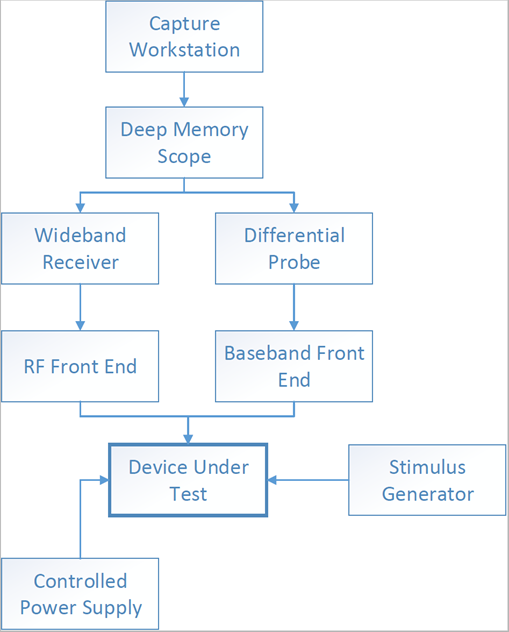
\includegraphics[width=1.0\linewidth]{images/chapter4/attacker_setup_schematic.png}
    \caption{Generic attack setup schematic} \label{fig:attack_setup_schematic}
\end{figure}

\Cref{fig:attack_setup_schematic} describes a generic power-analysis attack setup schematic.
We have the Device Under Test (DUT) connected to a very clean power supply (preferably a battery that gives a much cleaner supply of power than a standard AC/DC power supply). The ``Stimulus Generator'' is either a piece of software or hardware that allows us to automatically trigger the device's operation(s) we want to monitor. Then, we have the measurement front-end which is either a ``Baseband Front End'' i.e. a detour in the wiring conneced to a current/voltage proble or an ``RF Front End'' and a Wideband receiver for measuring the Electormagnetic field with good accuracy. The ``Deep Memory Scope'' is basically our oscilloscope that is capable of capturing lots of data very fast and transfer the digitized data to the ``Capture Workstation'' which is a very strong server or workstation that can handle the burden of thoroughly analysing the data to get the results we need.
This is quite a costly setup with cost in the range of hundreds of thousands of dollars, but once we have it in our lab - we can perform some very cool attacks!

\subsection { Research Highlights }

\begin{itemize}
    \item A nice paper provides a short biographical sketch of Ohm and a discussion of his experimental and theoretical work in general and ohm's law in specific \cite{gupta1980georg}.
    \item Stefan Mangard on his paper \cite{mangard2002simple} presents a simple power analysis attack on AES Implementation of the key expension.
    The attack, which performed on smart cards, exploit the infromation leaking during the AES key expansion, 
    and utilizes it to substantially reduce the key space that needs to be considered in a brute-force search for the secret key.
    \item W. Shan \cite{shan2017machine} presented a countermeasure to AES attack. the Algorithm porposed, based
    on maching learning, Wishes to find out the best hamming distance redistribution mapping to compensate the probability of hamming distance of the intermediate data directly,
    thus, make it unable to be distinguished from correct and incorrect sub-key.
    \item Another Paper posted on 2015 \cite{luo2015side} shows the weakneses of a very importanct component for running deep learning Algorithms, the GPU.
    The paper results, tested on NVIDIA TESLA GPU, shows that parallel computing hardware systems such as a GPU are highly vulnerable targets to power-based side-channel attacks,
    and survey some of the weakneses.
\end{itemize}


   
